\documentclass[11pt,a4paper]{article}

%\documentclass[11pt,a4paper]{IEEEtran}

%load packages
\usepackage{cite}
\usepackage{amsmath,amssymb,amsfonts}
\usepackage{algorithmic}
\usepackage{graphicx}
\usepackage{textcomp}
\usepackage{xcolor}
\usepackage[utf8]{inputenc}
\usepackage[british]{babel}
\usepackage[utf8]{inputenc}
\usepackage[acronym]{glossaries}
\usepackage[normalem]{ulem}
\usepackage{geometry}
\usepackage{minted}
\usepackage{soul}
\usepackage{array}

\usepackage{multicol}
\graphicspath{ {figures/} }
\usepackage{hyperref}
\hypersetup{
  colorlinks=false,
  linkcolor=true,
  filecolor=none,      
  urlcolor=none,
}
\urlstyle{same}
\geometry{
 a4paper,
 total={170mm,257mm},
 left=20mm,
 top=20mm,
}

% Prepare our glossary
\makeglossaries
\newacronym{ai}{AI}{Artificial Intelligence}
\newacronym{ml}{ML}{Machine Learning}
\newacronym{usd}{USD}{United States Dollar}
\newacronym{svm}{SVM}{Support Vector Machine}
\newacronym{mae}{MAE}{Mean Absolute Error}
\newacronym{mse}{MSE}{Mean Squared Error}
\newacronym{rmse}{RMSE}{Root Mean Squared Error}
\newacronym{pca}{PCA}{Principal Component Analysis}
\newacronym{pii}{PII}{Personally Identifiable Information}
\newacronym{knn}{k-NN}{k-Nearest Neighbors}
\newacronym{rfr}{RFR}{Random Forest Regressor}
\newacronym{gnb}{GBR}{Gradient Boosting Regressor}

% Define mathematical elements
\DeclareUnicodeCharacter{221D}{\ensuremath{∝}}
\DeclareUnicodeCharacter{220F}{\ensuremath{∏}}
\DeclareUnicodeCharacter{2223}{\ensuremath{∣}}


% Define Keywords and new commands
\newcommand{\hint}[1]{%
  \begingroup
  \sethlcolor{yellow!30}%
  \hl{#1}%
  \endgroup
}
\newcommand{\SubItem}[1]{
  {\setlength\itemindent{13pt} \item[◦] #1}
}
\newcommand{\SubSubItem}[1]{
  {\setlength\itemindent{26pt} \item[◦] #1}
}
\newcommand{\subsubsubsection}[1]{
  {\setlength\itemindent{13pt} \textit{\uline{\\#1\\}}} 
}
\def\keywords{\section*{Keywords}}


% \renewcommand{\listfigurename}{List of Figures}
% \renewcommand{\listtablename}{List of Tables}
% \renewcommand{\listoflistingscaption}{List of source codes}

% Lets start the whole document
\begin{document}
\title{Data scientists and machine learning \\
specialists salary prediction}
% \subtitle{Assignment in ICS 5110}
% \numberofauthors{4} 

\author{% enter a tabular-like environment
Danou Nauck \\
Aurora Court, Appartment 7\\
4 Triq Il-Vittem Tal-Gwerra\\
Haz-Zebbug ZBG 1295, Malta\\
\href{mailto:danou.nauck.24@um.edu.mt}{danou.nauck.24@um.edu.mt} \\ \\
Owen Gauci \\
Institute for Clarity in Documentation\\
P.O. Box 1212\\
xyz, Malta\\
\href{mailto:owen.gauci.24@um.edu.mt}{owen.gauci.24@um.edu.mt}  \\ \\
\and % switch to a new column
Paolo Fidicaro \\
Laboratories\\
National Lab\\
xyz, Malta\\
\href{mailto:paolo.fidicaro.24@um.edu.mt}{paolo.fidicaro.24@um.edu.mt} \\ \\
Ivan Ciancio \\
The TEGroup\\
1 Thircle\\
xyz, Malta \\ 
\href{mailto:ivan.ciancio.01@um.edu.mt}{ivan.ciancio.01@um.edu.mt} \\ \\
}

\IEEEoverridecommandlockouts
\author{\IEEEauthorblockN{John Albert\IEEEauthorrefmark{1}}
\IEEEcompsocitemizethanks{\IEEEcompsocthanksitem\IEEEauthorrefmark{1}equal contribution}
\IEEEauthorblockA{\textit{Dept. of CS} \\
 \textit{YYY University}\\
 City, Country \\
 Author1@email.com}
\and
\IEEEauthorblockN{author2} \\
\IEEEauthorblockA{Author2@email.com}
\and
\IEEEauthorblockN{author3} \\
\IEEEauthorblockA{Author3@email.com}
\and
\IEEEauthorblockN{autor4} \\
\IEEEauthorblockA{Author4@email.com}
}


% Lets start the real document
\maketitle
\begin{abstract}
This paper proposes a study to predict the salary of IT professionals working in the Artificial Intelligence, Machine learning and Data Science/Engineering areas given a set of features associated with individuals, using supervised machine learning approaches. The study has been conducted using a dataset that spreads from 2020 to 2022, therefore including also the effects of the Covid-19 pandemic on the job market. The dataset is based on 565 IT professionals with different job titles and working remotely, hybrid or on-site for companies located in different countries globally. \\
Both classification (such as Gaussian Naive Bayes and k-Nearest Neighbours classifier) and regression (such as Gradient Boosting regressor, Random forest and Support Vector Machine) techniques have been used for the implementation of prediction models. The \acrshort{knn} classifier overall measures outperformed the Gaussian Naive Bayesian algorithm with a predictive accuracy rate of 0.76, a precision of 0.77, a recall of 0.75 and F1-score of 0.74.

\end{abstract}

\keywords{AI, Salary, Prediction, Data Scientist, Machine Learning, Expert}

\section{Introduction}
The educational path we have undertaken might open new career opportunities in the \acrfull{ai}, \acrfull{ml} and Data Science/Engineering job market. It is interesting to analyze data regarding these job opportunities in order to find out what hopefully we could expect in the near future and how to guide our decisions in order to get the best out of it.
\hint{Among the three regression models, the XXXX outperformed YYY and ZZZZ with CCCC.}

For this purpose, we have selected the following dataset: \href{https://www.kaggle.com/datasets/ruchi798/data-science-job-salaries}{\textbf{Data Science Job Salaries}} that has the following properties:


\subsection{Data size} 
\begin{itemize}
\item \textbf{Number of Samples:} the initial dataset has 607 entries;
\item \textbf{Dimensionality:} the initial dataset has 12 features.
\end{itemize}

\subsection{Data Types} 
\begin{itemize}
\item \textbf{Numerical features:} 
\SubItem{\textbf{\texttt{ID}} - Unique numerical identifier of the entry;}
\SubItem{\textbf{\texttt{Salary\_in\_USD}} - The total gross salary in \acrfull{usd} (FX rate divided by avg. USD rate for the respective year via fxdata.foorilla.com);}
\SubItem{\textbf{\texttt{Salary}} - The total gross salary amount paid in the salary currency.}
\item \textbf{Categorical features:} 
\SubItem{\textbf{Work Year} - The year the salary was paid (2020, 2021 and 2022);}
\SubItem{\textbf{Experience level} - The experience level in the job during the year with the following possible values:}
\SubSubItem{\textbf{EN} - for Entry-level / Junior;}
\SubSubItem{\textbf{MI} - for Mid-level / Intermediate;}
\SubSubItem{\textbf{SE} - for Senior-level / Expert;}
\SubSubItem{\textbf{EX} - for Executive-level / Director;}
\SubItem{\textbf{Employee type} - The type of employment for the role:}
\SubSubItem{\textbf{PT} - for Part-Time;}
\SubSubItem{\textbf{FT} - for Full-Time;}
\SubSubItem{\textbf{CT} - for Contract;}
\SubSubItem{\textbf{FL} - for Freelance;}
\SubItem{\textbf{Job title} - The role worked during the year: 50 different job titles belonging to Artificial Intelligence, Machine learning and Data Science sectors. This is the only feature with free-form text;}
\SubItem{\textbf{Salary Currency} - The currency of the salary paid as an ISO 4217 currency code: 17 different currencies;}
\SubItem{\textbf{Employee residence} - Employee's primary country of residence during the work year as an ISO 3166 country code: 57 different countries of residence;}
\SubItem{\textbf{Company location} - The country of the employer's main office or contracting branch as an ISO 3166 country code: 50 different countries where the companies are located;}
\SubItem{\textbf{Company size} - The average number of people that worked for the company during the year: }
\SubSubItem{\textbf{S} - for companies with less than 50 employees (small);}
\SubSubItem{\textbf{M} - for companies with headcounts between 50 and 250 (medium);}
\SubSubItem{\textbf{L} - for companies with more than 250 employees (large);
}
\SubItem{\textbf{Remote ratio} - The overall amount of work done remotely, possible values are as follows:}
\SubSubItem{\textbf{0} - for on-site positions, with less than 20\% of remote work;}
\SubSubItem{\textbf{50} - for partially remote positions;}
\SubSubItem{\textbf{100} - for positions with more than 80\% remote work.}
\end{itemize}


\subsection{Feature Properties} 
\begin{itemize}
\item \textbf{Redundancy:} the \texttt{Salary} and the \texttt{Salary\_in\_USD} features are obviously highly correlated and provide duplicate information. For this reason, in the data preparation stage, it has been decided to remove the \texttt{Salary} and \texttt{Salary\_Currency} features from the dataset and to keep only the \texttt{Salary\_in\_USD} feature as target feature;
\item \textbf{Missingness:} There are NO missing or null values in the dataset;
\item \textbf{Duplicates:} If the \texttt{ID} feature is NOT considered, there are \uline{42 duplicated entries} in the dataset;
\item \textbf{Relevance:} Considering that the \texttt{Salary\_in\_USD} feature is the target feature (for regression models),  excluding the \texttt{ID} feature, that doesn’t add any information to the prediction, and removing the \texttt{Salary} and \texttt{Salary\_Currency} features because redundant, the mutual information calculated for each pair of the remaining features indicates that the \uline{features are mostly independent between each other}. The heatmap highlights that there is a correlation between feature 4 (employee residence) and 6 (company location), due to the fact that the majority of the employees is resident in the same country where the company they work for is located;

\begin{figure}
    \centering
    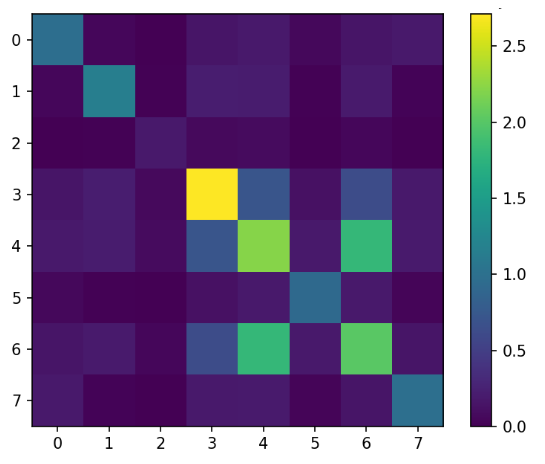
\includegraphics[width=1\linewidth]{ICS-5110-Fig-01.png}
    \caption{Mutual information between each pair of features}
    \label{fig:Mutual information between each pair of features}
\end{figure}

The following table displays the mutual information between each feature and the target feature (\texttt{Salary\_in\_USD}) and highlights that the following \uline{features contribute more to the prediction of the target: job title, employee residence and company location}.

\begin{table*}
\centering
\begin{tabular}{p{0.2\linewidth} | p{0.06\linewidth}| p{0.09\linewidth}| p{0.075\linewidth}| p{0.075\linewidth}| p{0.075\linewidth}| p{0.075\linewidth}| p{0.075\linewidth}| p{0.075\linewidth}} \hline
Feature no.&0&1&2&3&4&5&6&7\\ \hline
Feature Name&Work Year&Experience level&Employ- ment type&\textbf{Job title}&\textbf{Employee residence}&Remote ratio&\textbf{Company location}&Company size\\ \hline
Mutual information between the features and the target&0.76&0.87&0.14&\textbf{2.21}&\textbf{2.01}&0.69&\textbf{1.87}&0.71\\
\hline\end{tabular}
\caption{Mutual information between the features and the target}
\label{tab:Mutual information between the features and the target}
\end{table*}

\item \textbf{Target feature statistical distribution:} These are the statistical properties of the dataset
\SubItem{Mean of the salary in USD = 110,610.34 USD;}
\SubItem{Standard Deviation = 72,216.71 USD;}
\SubItem{Skewness = 1.728 (when Skewness $>$ 0 then there is more weight in the left tail of the distribution);}
\SubItem{Kurtosis = 6.384 (when the kurtosis $>$latex  3 the distribution is leptokurtic, this means that it tries to produce more outliers compared to the normal distribution);}
\SubItem{The dataset has also an evident outlier (see Figures 2 and 3) with a salary of 600,000 USD (a full-time Executive position in an American company).}

\begin{figure}
    \centering
    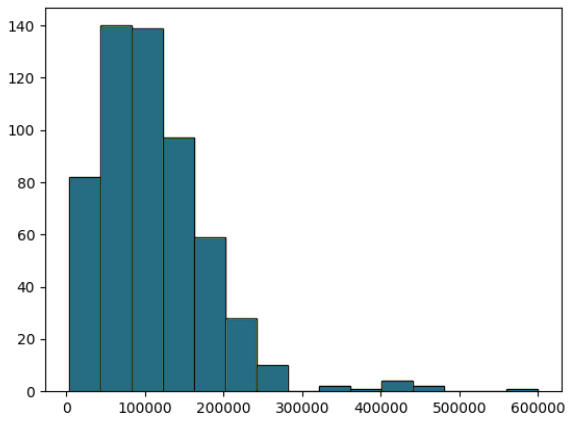
\includegraphics[width=1\linewidth]{ICS-5110-Fig-02.png}
    \caption{Salary in USD distribution}
    \label{fig:Salary in USD distribution}
\end{figure}

\begin{figure}
    \centering
    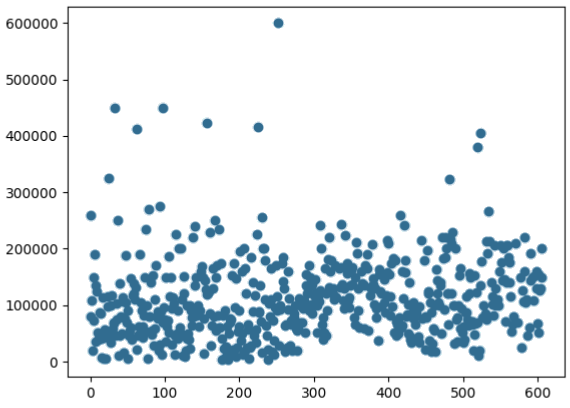
\includegraphics[width=1\linewidth]{ICS-5110-Fig-03.png}
    \caption{Plot distribution of the salaries in USD}
    \label{fig:Plot distribution of the salaries in USD}
\end{figure}

\item \textbf{Imbalance:}
\SubItem{\textbf{Years} - the year categorical feature has an uneven distribution with a greater number of samples in 2021 and 2022 compared to 2020;}

\begin{figure}
    \centering
    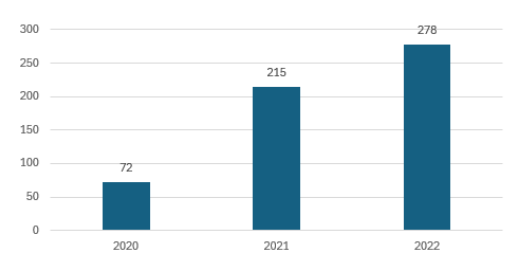
\includegraphics[width=1\linewidth]{ICS-5110-Fig-04.png}
    \caption{Distribution of the samples per year}
    \label{fig:Distribution of the samples per year}
\end{figure}

\SubItem{\textbf{Experience level} - the experience level categorical feature has an uneven distribution, however, it follows a normal distribution that can be expected in a company (a few executives, a small number of entry levels and the majority of middle positions);}

\begin{figure}
    \centering
    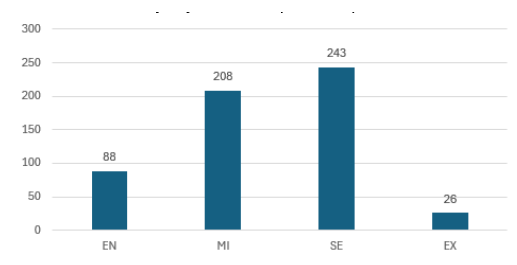
\includegraphics[width=1\linewidth]{ICS-5110-Fig-05.png}
    \caption{Distribution of the samples per experience level}
    \label{fig:Distribution of the samples per experience level}
\end{figure}

\SubItem{\textbf{Employee type} - the type of employment categorical feature has an uneven distribution strongly centered on Full-time employees (546), with just a few part-timers (10), contractors (5) and freelancers (4);}
\SubItem{\textbf{Job Title} - there are 50 different job titles and the distribution is uneven having the majority of samples belonging to the following 4 job titles: Data scientist (130), Data Engineer (121), Data analyst (82) and Machine learning engineer (39);}
\SubItem{\textbf{Company size} - the company size  categorical feature has an uneven distribution, however, it follows a normal distribution that can be expected in the IT market;}

\begin{figure}
    \centering
    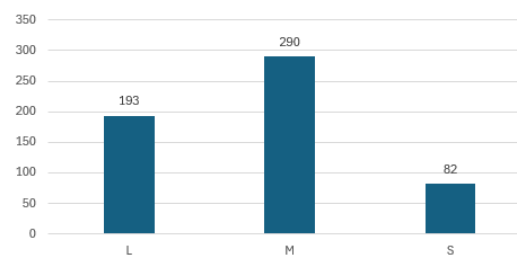
\includegraphics[width=1\linewidth]{ICS-5110-Fig-06.png}
    \caption{Distribution of the samples per company size}
    \label{fig:Distribution of the samples per company size}
\end{figure}

\SubItem{\textbf{Employee residence} - the employees are distributed among 57 different countries, however the distribution is uneven and it is mainly centered on USA (295), Great Britain (43), India (30), Canada (27), Germany (24);}
\SubItem{\textbf{Company location} - the companies are distributed among 50 different countries, however the distribution is uneven and it is mainly centered on USA (318), Great Britain (46), Canada (28), Germany (27), India (24);}
\SubItem{\textbf{Remote ratio} - the remote ratio categorical feature has an uneven distribution with the majority of remote positions. This is in line with the trend that was in place from 2020 to 2022, during and immediately after the Covid-19 period. This trend has been inverted in recent years, so this distribution might be different if we consider the years 2023 and 2024;}
\SubItem{\textbf{Salary Group} - n the data preparation stage, a new feature \texttt{Salary\_Group} has been introduced to group the entries in 3 salary categories (Low, Medium and High). In order to have an even distribution of this new categorical feature, that can be used for categorical prediction models, the entries have been divided considering two thresholds:}
\SubSubItem{\textbf{33 percentile} of the salary in USD = 74,015.6 USD;}
\SubSubItem{\textbf{66 percentile} of the salary in USD = 128,875.0 USD}
Therefore the \texttt{Salary\_Group} values are defined based on the following logic:
\SubSubItem{\textbf{\texttt{Salary\_Group} = L (low)} if the \texttt{Salary\_in\_USD} $<$ 74,015.6}
\SubSubItem{\textbf{\texttt{Salary\_Group} = M (medium)}  if the 74,015.6 $<$= \texttt{Salary\_in\_USD} $<$  128,875.0}
\SubSubItem{\textbf{\texttt{Salary\_Group} = H (high)} if the \texttt{Salary\_in\_USD} $>$= 128,875.0}
\end{itemize}

\subsection{Analysis plan} 
The purpose of this analysis is to:
\begin{itemize}
\item Identify the features that directly influence the salary amount (regression) or salary category (categorization);
\item Reply to the following research questions:
\SubItem{\textbf{What is the average data scientist salary?} - the mean value of the salary in USD is 110,610.34 USD;}
\SubItem{\textbf{What is the most popular job title in data science?} - the most popular job title is Data scientist (130), followed by Data Engineer (121) and Data analyst (82);}
\SubItem{\textbf{Which country has better opportunities for data science jobs?} - the country with most opportunities for data science jobs is USA;}
\SubItem{\textbf{How many employees at each seniority level?} - there are 88 entry-level, 208 mid-level, 243 senior and 28 Executive positions;}
\SubItem{\textbf{How many employees work remotely?} -  majority of the employees work remotely (346), however, it has to be considered that the dataset is from 2020 and 2022, when the remote job trend was still strong;}
\SubItem{\textbf{Do small companies pay data scientists and machine learning engineers more than large companies?} - No, the average salary with small companies (77,872.1 USD) is smaller than the average salary with large companies (118,213.1 USD);}
\SubItem{\textbf{Does the job title have a relevant role in determining the salary?} - Yes, the job title is the most relevant feature to determine the salary. The mutual information between the job title and the Salary amount is the highest among all the features (2.21) - see Table 1;}
\SubItem{\textbf{Are remote opportunities paid less than on-site/hybrid ones?} - No, fully remote jobs were paying more than on-site or hybrid ones, however, we must consider that the dataset refers to the years 2020, 2021 and 2022, when the effect of Covid-19 on our society were predominant and when we were forced into remote jobs;}
\SubItem{\textbf{Which type of employment and which company size are better for an entry level?} - for a person with entry level work experience in the field, the best type of employment is as Contractor for Large companies, with an average salary of 100,000 USD compared to an average salary of 61,643.32 USD for entry level experience considering ALL types of companies in terms of size;}
\item Identify the optimal prediction model for predicting the salary amount or the salary category among selected participant segments.
\end{itemize}
These are the Machine Learning techniques that have been used for the prediction analysis:
\begin{itemize}
\item \textbf{Regression:}
\SubItem{Gradient Boosting regressor}
\SubItem{Random forest }
\SubItem{\acrfull{svm}}
\item \textbf{Multiclass classification:}
\SubItem{Gaussian Naive Bayesian classifier}
\SubItem{K-Nearest Neighbour classifier}
\end{itemize}
These are the metrics that will be used to measure the performance of each ML method applied and to compare the regression models and the classification models with each other:
\begin{itemize}
\item \textbf{Regression:}
\SubItem{\acrfull{mae}}
\item \textbf{Multiclass classification:}
\SubItem{Confusion Matrix}
\SubItem{Accuracy ratio}
\SubItem{Precision, Recall, and F1-score}
\end{itemize}

\section{Background}
\subsection{Rescaling and normalisation} 
Rescaling and normalization are data preprocessing techniques that modify the scale or distribution of features in a dataset to improve the performance and efficiency of machine learning models. These methods ensure that features contribute proportionately to the model training process, particularly when different features have vastly different ranges or units.
\\
Rescaling adjusts the range of feature values to a fixed interval, typically [0, 1] or [-1, 1]. The simplest rescaling algorithm is the Min-Max scaling that is calculated as:

\begin{displaymath}
X' = \frac{(X - Xmin)}{(Xmax - Xmin)}  
\end{displaymath}

Where:
\begin{itemize}
\item \textbf{X} is the original feature value.
\item \textbf{Xmin} and \textbf{Xmax} are the minimum and maximum values of the feature.
\end{itemize}
The rescaling ensures all features have the same scale, which can be important for algorithms sensitive to feature magnitude (e.g., k-Nearest Neighbors or \acrshort{svm}s), so doing it prevents features with larger ranges from dominating the optimization process.
\\
Normalization (or standardization) transforms feature values to have a mean of 0 and a standard deviation of 1. It is achieved using the formula:

\begin{displaymath}
X' = \frac{(X - \mu)}{\sigma}  
\end{displaymath}

Where:
\begin{itemize}
\item \textbf{X} is the original feature value.
\item $\boldsymbol{\mu}$ is the mean of the feature.
\item $\boldsymbol{\sigma}$ is the standard deviation of the feature. 
\end{itemize}
Normalized data is centered around zero and scales it by variability, which is crucial for algorithms that assume normally distributed data (e.g., linear regression, logistic regression or \acrfull{pca}). Normalization speeds up gradient-based optimization algorithms by providing faster convergence.
\\
Rescaling and normalization are important because:
\begin{itemize}
\item they improve models performances, especially for optimization algorithms.
\item ensure a balanced contributions of the feature, preventing features with large ranges from dominating smaller-scale features.
\item for models like \acrshort{svm} or logistic regression, normalized data ensures that hyperplanes or decision boundaries are calculated correctly.
\end{itemize}
\subsection{Cross-validation} 
Cross-validation is a statistical technique used to evaluate the performance of a machine learning model. It helps ensure that the model is not overfitting or underfitting by testing it on different subsets of the data.
\\
There are several types of cross-validations. The one we are going to use for some of our experiments is the K-fold cross-validation that is implemented by dividing the dataset into k subsets and iteratively using each subset as a validation (testing) set and the remaining subsets as training set. For each iteration, once the model is trained, the performance metrics are calculated and stored and the model is discarded. The performance metrics (e.g., accuracy, precision, recall) from all iterations are averaged to provide an overall assessment of the model's performance. 
\\
Cross-validation helps in reducing the risk of overfitting to a single train-test split and provides a more comprehensive evaluation of model performance.
\subsection{Dimensionality reduction and feature selection} 
Dimensionality reduction is a transformation process that allows to reduce the number of input features for the prediction model; whereas, the feature selection is a method of identification of the features of the dataset that retain as much relevant information as possible and using only these features in the prediction model.
\\
Both processes reduce the computational load and allow the visualization of the dataset, in case of reduction to or selection of 1 or 2 features (excluding the target feature).
\\
The features have to be selected so that they are independent of each other and are highly dependent on the target variable to be predicted.
The feature selection has been applied to the dataset by removing:

\begin{itemize}
\item The \texttt{Salary} and \texttt{Salary\_Currency} features because redundant considering that the out target feature is the \texttt{Salary\_in\_USD} 
\item The \texttt{ID} feature that doesn’t add any information to the prediction
\end{itemize}

The mutual information calculated for each pair of the remaining features indicates that they are independent between each other (see Fig.1 above).
\subsection{Performance evaluation metrics} 
These are the metrics that will be used to measure the performance of each ML method applied and to compare the regression models and the classification models with each other:
\begin{itemize}
\item \textbf{Regression}
\SubItem{The \acrfull{mae} measures the average absolute difference between the predicted values and the actual target values. Unlike other metrics, MAE doesn’t square the errors, which means it gives equal weight to all errors, regardless of their direction.}
\begin{displaymath}
MAE = \frac{1}{N} \sum_{i=1}^{N} | y_i  - \hat{y} | 
\end{displaymath}
\SubItem{The \acrfull{mse} represents the average of the squared difference between the original and predicted values in the data set.}
\begin{displaymath}
MSE = \frac{1}{N} \sum_{i=1}^{N} (y_i  - \hat{y})^2
\end{displaymath}
\SubItem{The \acrfull{rmse} is the square root of \acrshort{mse}.}
\begin{displaymath}
RMSE = \sqrt{MSE} = \sqrt{ \frac{1}{N} \sum_{i=1}^{N} (y_i  - \hat {y})^2}
\end{displaymath}
\item \textbf{Multiclass classification}
\SubItem{\textbf{Confusion Matrix} → the confusion matrix is a concise representation of the number of correct and incorrect predictions made by a prediction model. The Confusion matrix visualizes the performance of the multi-class classification model by comparing predicted and actual class labels for the dataset and it is used as base for calculating the other performance metrics of a multi-class classification model.
\begin{figure*}
    \centering
    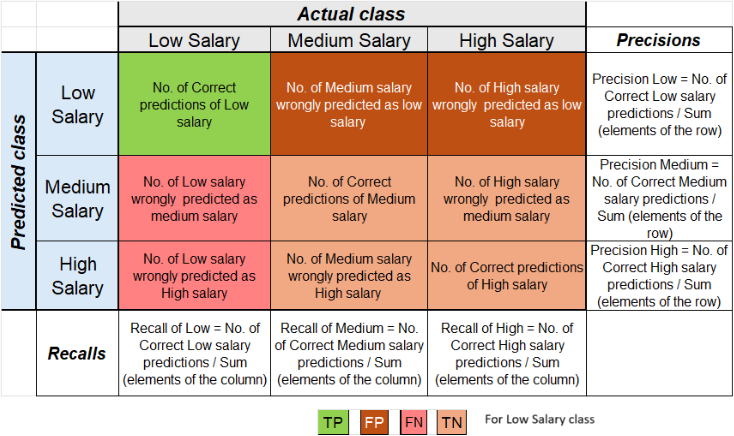
\includegraphics[width=1\linewidth]{ICS-5110-Table-02.png}
    \caption{Multiclass (3-class) Confusion matrix for the Low Salary class and description of TP,TN, FP and FN}
    \label{fig:Multiclass (3-class) Confusion matrix for the Low Salary class}
\end{figure*}
\\
The True positive, True negative, False positive and False negative values must be calculated separately for each class. Table 2 depicts how the 3-class Confusion matrix is populated and how to determine the TP, FP, TN and FN for the Low Salary class: the row of the predicted Low salaries class (1st row) identifies the positives, whereas the remaining 2 rows identify the negatives; the true predictions are the correct ones;}
\SubItem{\textbf{Accuracy rate} → the Accuracy rate is calculated from the values of the Confusion matrix by considering the sum of the Correct elements at the numerator (sum of the values in the diagonal of the Confusion matrix) and the sum of all the entries of the confusion matrix at the denominator (both correct and incorrect predictions).}
\begin{displaymath}
Accuracy = \frac{Correct\ predictions}{All\ predictions} 
\end{displaymath}
The Accuracy metric measures how much the model is correctly predicting on the set of data assuming that each unit contributes equally to the Accuracy value;
\SubItem{\textbf{Recall} → the Recall metric, also called Sensitivity, measures how many relevant items have been correctly found for each class, how many of the actual positive items our model correctly has identified:}
\begin{displaymath}
Recall_{class} = \frac{TP_{class}}{TP_{class} + FN_{class}} 
\end{displaymath}
The overall Recall metric of the model can be calculated through micro-averaging or macro-averaging. The 3 classes of salary are well balanced, because they have been defined by using the 33 and 66 percentiles of the target feature distribution, therefore a macro-averaging value can be used to calculate the overall Recall value of the model:
\begin{displaymath}
Recall = \frac{Recall_{Low}\ + Recall_{Medium}\ + Recall_{High}}{3} 
\end{displaymath}

\SubItem{\textbf{Precision} → the Precision metric measures how many of the items our model has predicted as positive were actually positive for each class:}
\begin{displaymath}
Precision_{class} = \frac{TP_{class}}{TP_{class} + FP_{class}} 
\end{displaymath}
The overall Precision metric of the model can be calculated through micro-averaging or macro-averaging. The 3 classes of salary are well balanced, because they have been defined by using the 33 and 66 percentiles of the target feature distribution, therefore a macro-averaging value can be used to calculate the overall Precision value of the model:
\begin{displaymath}
Precision = \frac{Pr_{Low}\ + Pr_{Medium}\ + Pr_{High}}{3} 
\end{displaymath}
\SubItem{\textbf{F1-score} → the F1-score is a measure that combines recall and precision in a harmonic mean where both measures are equally weighted. There is a trade-off to be handled between precision and recall, F1 can therefore be used to measure how effectively our models make that trade-off:}
\begin{displaymath}
F1-score = 2 * \frac{Precision * Recall}{Precision + Recall} 
\end{displaymath}
\end{itemize}
\section{Data Preparation} 
These are the steps executed to process the dataset and prepare it for the individual experiments with different prediction models:
\begin{itemize}
\item Removal of duplicates
\item Feature selection
\item Data pre-processing
\SubItem{Generation of a new target feature for Classification models} 
\SubItem{Transformation of Categorical Features to Numerical Values}
\SubSubItem{Rescaling of numerical values}
\item Data splitting between training and test and cross-validation
\end{itemize}
\subsection{Removal of duplicates} 
There are \uline{42 duplicated entries} in the dataset (NOT considering the ID feature). Duplicated data points might be:
\begin{itemize}
\item Correct data that happen to be the same for more than one occurrence, in this case these true points should be taken in consideration since they are part of the overall phenomenon under analysis
\item Actual duplications of data points that have been incorrectly added to the dataset, in this case these data points must be dropped because they don’t add any information to the model, and they can skew the model reinforcing specific behaviours
\end{itemize}
It is NOT possible to determine which of the above scenarios we are facing, therefore, keeping a conservative approach, it has been decided to remove the duplicates. \uline{The cleaned dataset has been reduced from 607 to 565 unique entries.}
\subsection{Feature selection} 
The dataset has 12 different features (see the Introduction section for more details).
The \texttt{Salary} and the \texttt{Salary\_in\_USD} features are obviously highly correlated and provide duplicate information. For this reason, it has been decided to remove the Salary and \texttt{Salary\_Currency} features from the dataset and keep only the \texttt{Salary\_in\_USD}, in order to have all the data points with the same currency.
\\
The ID feature isn’t relevant for the data analysis so it has been removed as well. \textbf{The dataset has been reduced to 9 features}, one of which is the target feature (\texttt{Salary\_in\_USD}).
\\
The mutual information calculated for each pair of these remaining 9 features indicates that the \uline{features are mostly independent between each other}. There is a small correlation between feature 4 (employee residence) and 6 (company location), due to the fact that the majority of the employees is resident in the same country where the company they work for is located, however it has been considered important to keep both features because they carry different type of characterization of the data points.  


\subsection{Data preprocessing - new feature generation} 
The Data preprocessing includes the generation of a new target feature for Classification models. The dataset can be used for:
\begin{itemize}
\item Predicting the annual salary in USD for jobs in the Data science/ Machine learning area → REGRESSION problem;
\item Predicting the range of annual salary in USD for jobs in the Data science/ Machine learning area – MULTI-CLASS CLASSIFICATION problem.
\end{itemize}

A new feature (\texttt{Salary\_Range}) has been introduced to enable the dataset to Classification prediction model.

The dataset can be split in 3 categories of salaries, High, Medium and Low. In order to have balanced categories of salaries, the thresholds that define the extreme of the salary ranges can use the 33th and the 66th percentile of the distribution:
\begin{itemize}
\item The 33$^{th}$ percentile of the distribution is 74,015.6 USD
\item The 66$^{th}$ percentile of the distribution is 128,875.0 USD
\end{itemize}
The \texttt{Salary\_Group} feature is added to the dataset based on the following rules:
\begin{itemize}
\item \textbf{Low salaries (L)} are the ones below 74,015.6 USD → 187 data points
\item \textbf{Mid salaries (M)} are the ones between 74,015.6 USD and 128,875.0 USD → 185 data points
\item \textbf{High salaries (H)} are the ones above 128,875.0 USD → 193 data points
\end{itemize}

\subsection{Data preprocessing - feature transformation} 
Transformation of Categorical Features to Numerical Values and rescaling
Categorical features must be transformed into numerical values in order to make use of machine learning libraries in Python. Several techniques can be applied to perform such transformation: ordinal encoding (the categories are simply numbered sequentially 1, 2, 3…), one-time encoding (an n-dimensional vector, where n is the number of possible values of the category, with binary values represents each category value), target encoding (each category is replaced by the mean value of the target variable for that category). The target encoding method is applied in this project because there is a strong relationship between the target variable and the categorical variables.
\\
After the transformation to numerical values, the features values are rescaled. Here is the mapping of the categorical features values with their numerical values and the rescaled values.
\\

\begin{table}
\centering
\begin{tabular}{p{0.15\linewidth}|p{0.50\linewidth}|p{0.15\linewidth}|p{0.10\linewidth}} \hline
\textbf{Categor-ical feature}&\textbf{Categorical feature value}&\textbf{Numerical value} (average of categorical salaries)&\textbf{Rescaled value}\\ \hline
work&2020&95813.00&0\\
year&2021&99430.41&0.13\\
&2022&123089.09&1.0\\
\hline
experience&EN&61643.32&0\\
level&MI&87792.99&0.19\\
&SE&138374.88&0.56\\
&EX&199392.04&1.0\\
\hline
employ-&CT&184575.00&1.0\\
ment&FL&48000.00&0.1\\
type&FT&111811.84&0.52\\
&PT&33070.50&0\\
\hline
job title&3D Computer Vision Researcher&5409.00&0\\
&AI Scientist&66135.57&0.152\\
&Analytics Engineer&175000.00&0.424\\
&Applied Data Scientist&175655.00&0.426\\
&Applied Machine Learning Scientist&142068.75&0.341\\
&BI Data Analyst&74755.16&0.173\\
&Big Data Architect&99703.00&0.235\\
&Big Data Engineer&51974.00&0.116\\
&Business Data Analyst&76691.20&0.178\\
&Cloud Data Engineer&124647.00&0.298\\
&Computer Vision Engineer&44419.33&0.097\\
&Computer Vision Software Engineer&105248.66&0.250\\
&Data Analyst&90089.59&0.211\\
&Data Analytics Engineer&64799.25&0.148\\
&Data Analytics Lead&405000.00&1.0\\
&Data Analytics Manager&127134.28&0.304\\
&Data Architect&177873.90&0.431\\
&Data Engineer&109750.03&0.261\\
&Data Engineering Manager&123227.20&0.294\\
&Data Science Consultant&69420.71&0.160\\
&Data Science Engineer&75803.33&0.176\\
&Data Science Manager&158328.50&0.382\\
&Data Scientist&103336.35&0.245\\
&Data Specialist&165000.00&0.399\\
&Director of Data Engineering&156738.00&0.378\\
&Director of Data Science&195074.00&0.474\\
&ETL Developer&54957.00&0.123\\
&Finance Data Analyst&61896.00&0.141\\
&Financial Data Analyst&275000.00&0.674\\
&Head of Data&160162.60&0.387\\
&Head of Data Science&146718.75&0.353\\
&Head of Machine Learning&79039.00&0.184\\
&Lead Data Analyst&92203.00&0.217\\
&Lead Data Engineer&139724.50&0.336\\
&Lead Data Scientist&115190.00&0.274\\
&Lead Machine Learning Engineer&87932.00&0.206\\
&ML Engineer&117504.00&0.280\\
&Machine Learning Developer&85860.66&0.201\\
&Machine Learning Engineer&101165.12&0.240\\
&Machine Learning Infrastructure Engineer&101145.00&0.239\\
&Machine Learning Manager&117104.00&0.279\\
&Machine Learning Scientist&158412.50&0.383\\
&Marketing Data Analyst&88654.00&0.208\\
&NLP Engineer&37236.00&0.079\\
&Principal Data Analyst&122500.00&0.293\\
&Principal Data Engineer&328333.33&0.808\\
&Principal Data Scientist&215242.42&0.525\\
&Product Data Analyst&13036.00&0.019\\
&Research Scientist&109019.50&0.259\\
&Staff Data Scientist&105000.00&0.249\\
\hline\end{tabular}
\caption{Transformation of Categorical Features to Numerical Values and rescaling}
\label{tab:Transformation of Categorical Features to Numerical Values}
\end{table}
\begin{table}
\centering
\begin{tabular}{p{0.15\linewidth}|p{0.18\linewidth}|p{0.15\linewidth}|p{0.10\linewidth}} \hline
\textbf{Categor-ical feature}&\textbf{Categorical feature value}&\textbf{Numerical value} (average of categorical salaries)&\textbf{Rescaled value}\\ \hline
employee&AE&100000.00&0.4896\\
residence&AR&60000.00&0.2857\\
&AT&76738.66&0.3711\\
&AU&108042.66&0.5308\\
&BE&85699.00&0.4168\\
&BG&80000.00&0.3877\\
&BO&75000.00&0.3622\\
&BR&54634.66&0.2583\\
&CA&97191.62&0.4754\\
&CH&122346.00&0.6038\\
&CL&40038.00&0.1838\\
&CN&43331.00&0.2006\\
&CO&21844.00&0.0910\\
&CZ&69999.00&0.3367\\
&DE&85336.66&0.4149\\
&DK&37252.50&0.1696\\
&DZ&100000.00&0.4896\\
&EE&32974.00&0.1478\\
&ES&57593.40&0.2734\\
&FR&59886.61&0.2851\\
&GB&81470.06&0.3952\\
&GR&56445.75&0.2675\\
&HK&66022.00&0.3164\\
&HN&20000.00&0.0816\\
&HR&45618.00&0.2123\\
&HU&35997.00&0.1632\\
&IE&71444.00&0.3441\\
&IN&37322.33&0.1700\\
&IQ&100000.00&0.4897\\
&IR&4000.00&0\\
&IT&61600.00&0.2938\\
&JE&100000.00&0.4898\\
&JP&103537.71&0.5078\\
&KE&9272.00&0.0268\\
&LU&59102.00&0.2811\\
&MD&18000.00&0.0714\\
&MT&28369.00&0.1243\\
&MX&18185.00&0.0723\\
&MY&200000.00&1.0\\
&NG&30000.00&0.1326\\
&NL&60956.60&0.2905\\
&NZ&125000.00&0.6173\\
&PH&45760.00&0.2130\\
&PK&27462.83&0.1197\\
&PL&56177.50&0.2662\\
&PR&160000.00&0.7959\\
&PT&42862.50&0.1982\\
&RO&51419.00&0.2419\\
&RS&25532.00&0.1098\\
&RU&105750.00&0.5191\\
&SG&104176.50&0.5111\\
&SI&63831.00&0.3052\\
&TN&31875.00&0.1422\\
&TR&20096.66&0.0821\\
&UA&13400.00&0.0479\\
&US&150094.91&0.7453\\
&VN&30800.00&0.1367\\
\hline
remote&0&105785.40&0.62\\
ratio&50&80721.89&0.00\\
&100&120763.19&1.00\\
\hline\end{tabular}
\caption{Categorical Features Of Residence and Remote Amount}
\label{tab:Categorical Features Of Residence and Remote Amount}
\end{table}
\begin{table}
\centering
\begin{tabular}{p{0.15\linewidth}|p{0.25\linewidth}|p{0.15\linewidth}|p{0.10\linewidth}} \hline
\textbf{Categor-ical feature}&\textbf{Categorical feature value}&\textbf{Numerical value} (average of categorical salaries)&\textbf{Rescaled value}\\ \hline
company&AE&100000.00&0.6254\\
location&AS&18053.00&0.0915\\
&AT&72920.75&0.4489\\
&AU&108042.66&0.6778\\
&BE&85699.00&0.5322\\
&BR&18602.66&0.0951\\
&CA&100121.85&0.6262\\
&CH&64114.00&0.3916\\
&CL&40038.00&0.2347\\
&CN&71665.50&0.4408\\
&CO&21844.00&0.1162\\
&CZ&50937.00&0.3057\\
&DE&81559.55&0.5052\\
&DK&54386.33&0.3282\\
&DZ&100000.00&0.6255\\
&EE&32974.00&0.1887\\
&ES&53060.14&0.3196\\
&FR&63970.66&0.3906\\
&GB&81649.50&0.5058\\
&GR&52026.70&0.3128\\
&HN&20000.00&0.1042\\
&HR&45618.00&0.2711\\
&HU&35735.00&0.2067\\
&IE&71444.00&0.4393\\
&IL&119059.00&0.7495\\
&IN&28581.75&0.1601\\
&IQ&100000.00&0.6256\\
&IR&4000.00&0.00\\
&IT&36366.50&0.2108\\
&JP&114127.33&0.7174\\
&KE&9272.00&0.0343\\
&LU&43942.66&0.2602\\
&MD&18000.00&0.0912\\
&MT&28369.00&0.1587\\
&MX&32123.33&0.1832\\
&MY&40000.00&0.2345\\
&NG&30000.00&0.1693\\
&NL&54945.75&0.3318\\
&NZ&125000.00&0.7882\\
&PK&13333.33&0.0608\\
&PL&66082.50&0.4044\\
&PT&47793750&0.2853\\
&RO&60000.00&0.3648\\
&RU&157500.00&1.00\\
&SG&89294.00&0.5556\\
&SI&63831.00&0.3897\\
&TR&20096.66&0.1048\\
&UA&13400.00&0.0612\\
&US&144292.99&0.9139\\
&VN&4000.00&0.01\\
\hline
company&L&118213.88&1.00\\
size&M&114807.07&0.91\\
&S&77872.09&0.00\\
\hline\end{tabular}
\caption{Categorical Features Of Company location and size}
\label{tab:Categorical Features Of Company location and size}
\end{table}

\subsection{Data splitting} 
Data splitting between training and test and cross-validation
\\
There are several types of cross-validations. The one used for some of our experiments is the K-fold cross-validation that is implemented by dividing the dataset into testing and training - validation subsets and then dividing further the the latter in k subsets and iteratively using each subset as a validation set and the remaining subsets as training set. For each iteration, once the model is trained, the performance metrics are calculated and stored and the model is discarded. The performance metrics (e.g., accuracy, precision, recall) from all iterations are averaged to provide an overall assessment of the model's performance. \\
Cross-validation helps in reducing the risk of overfitting to a single train-test split and provides a more comprehensive evaluation of model performance. \\
Standard training-validation-testing splitting or K-Fold cross-validation or both have been applied case by case. The decision of applying a K-Fold Cross-Validation has been taken in order to have a more reliable performance estimation and less risk of overfitting to the training data considering the reduced size of the dataset.

\section{Prediction models and experiments}
\subsection{K-Nearest Neighbour}
\subsubsection{Model description}
The \textbf{\acrfull{knn}} model is a supervised machine learning algorithm that can be applied to both classification and regression tasks. For this experiment, the model has been used as a classifier.\\
The k-NN method is a non-parametric algorithm that classifies data points based on their features representation and their “similarity” with their k closest neighbours in the feature space, assuming that similar data points are likely to have similar outcomes (target labels).
This algorithm doesn’t require any underlying distribution between features in order to be applied.  \\
The k-NN algorithm does not "train" a model in the traditional sense. Instead, it stores the entire training dataset and their label and classifies new cases based on a similarity measure. The algorithm is applied with a defined value of k, that is the number of nearest neighbours to include in the prediction process.\\
Once the whole training dataset D has been stored and its features normalized and/or standardized, the algorithm applies the following logic for classification problems:
\begin{itemize}
\item Computing of the distance between the data point to be predicted and all points in the training dataset $d(x',x_i)$ for every $x_i \in D$. There are different distance metrics that can be used, the most common are:
\SubItem{\textbf{Euclidean distance:}
\begin{displaymath}
d( x' , x_i ) = \sqrt{ \sum_{i=1}^{N} (x'  - x_i)^2}
\end{displaymath}}
\SubItem{\textbf{Manhattan distance:} 
\begin{displaymath}
d( x' , x_i ) = \sum_{i=1}^{N} |x'  - x_i|
\end{displaymath}}
\SubItem{\textbf{Gower’s distance:}
That can be used for different types of data
\begin{displaymath}
d(xi,xj) = \frac{ \sum_{i=1}^{N} (W_k * d_{ij})} {\sum_{i=1}^{N} (W_k)}
\end{displaymath}
where }
\begin{displaymath}
d_{ij} = \frac{∣ x_i - x_j ∣}{range_k}  
\end{displaymath} 
\SubSubItem{with $range_k$ the difference between the maximum and minimum values of the k.th variable in the dataset}
\SubSubItem{$W_k$ weight of the k.th variable in the dataset}
\item Identifying the k nearest neighbors of x' based on the calculated distances
\item Performing a majority vote among the k neighbors: the class with the most votes becomes the predicted class.
\end{itemize}
The algorithm is sensitive to scale, so features with larger scales dominate the distance calculations. The dataset for this experiment has already been rescaled and it has also been normalized before the experiments, making the application of the k-NN algorithm to the dataset more reliable. \\
The algorithm's performance depends on the choice of \textbf{k} and its effectiveness on the choice of distance metric.For the selection of the best value for \textbf{k}, the model is tested with multiple \textbf{k} values through cross-validation and finally the \textbf{k} value that maximizes the accuracy of the model is selected.

\subsubsection{Experiment execution}
The goal of the experiments was to evaluate the performance of the k-Nearest Neighbors (k-NN) classifier on the given dataset and to understand the effect of varying hyperparameters such as the number of neighbors (k) and distance metrics.\\
The data was already partially pre-processed before the execution of the experiments (see Data preparation section above): the data was rescaled and the categorical features transformed to numerical values. \\
An additional standardisation has been applied to the dataset in order to convert the statistical distribution of the data so to have mean = 0 and standard deviation = 1.
\\
\\
\textbf{I. Experiment initial settings and results - k-fold cross validation
The experiment started with the following setup:}
\begin{itemize}
\item \uline{The dataset has been split in training and test sets, with an 80/20 ratio, and the k-fold cross validation has been applied on the training set considering 5 folds};
\item The \uline{Euclidean distance} has been applied as distance metric;
\item All points in each neighborhood have been weighted equally.
\end{itemize}
The initial objective of the experiment was to assess the impact of k on the classificator’s accuracy applying a k-fold cross validation to the entire dataset. With an initial value of k-fold = 5 folds, the k-NN model has been applied to k (number of neighbours) values in the range [1, 361]. For each value of k, the average of the accuracies calculated for each folds’ permutations has been calculated. This is the resulting K - average accuracy distribution.
\begin{figure}
    \centering
    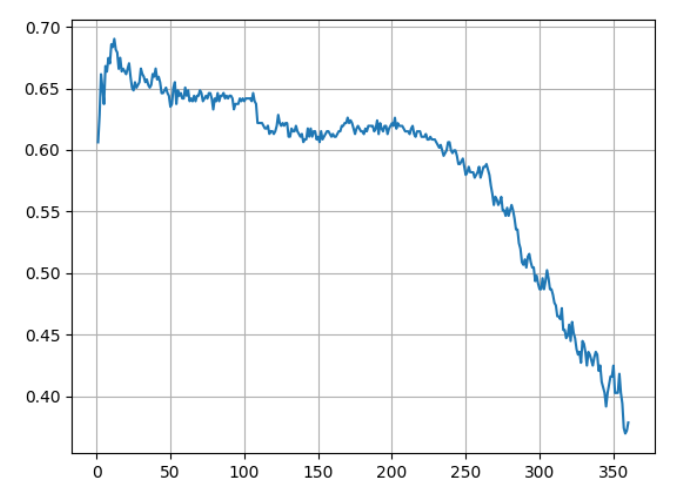
\includegraphics[width=1\linewidth]{ICS-5110-Fig-08.png}
    \caption{Average accuracy scores of the k-NN model with different k values through 5-folds cross-validation}
    \label{fig:Average accuracy scores of the k-NN model with different k values 5-fold}
\end{figure}
The max average accuracy is reached with \textbf{k = 11, with average accuracy of 0.69}.
The experiment has been executed again considering a value of k-fold = 10 folds, and applying the k-NN model to k (number of neighbours) values in the range [1, 361]. For each value of k, the average of the accuracies calculated for each folds’ permutations has been calculated. This is the resulting K - average accuracy distribution.
\begin{figure}
    \centering
    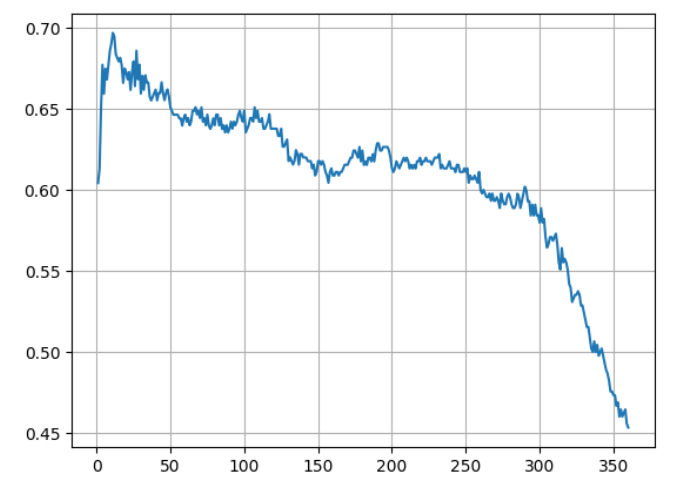
\includegraphics[width=1\linewidth]{ICS-5110-Fig-09.png}
    \caption{ Average accuracy scores of the k-NN model with different k values through 10-folds cross-validation }
    \label{fig:Average accuracy scores of the k-NN model with different k values 10-fold}
\end{figure}
Increasing the number of folds of the cross validation to \textbf{10 folds}, the max average accuracy is reached with \textbf{k = 10, with average accuracy of 0.69 and F1-score = 0.68}. No relevant improvements of the model average accuracy have been achieved by doubling the number of folds in the cross-validation.
\\
\\
\textbf{II. Dataset split in training, validation and testing sets (70\%, 10\% , 20\%) - configuration evaluation against validation set:}
The experiment has been continued to investigate how a standard split of the dataset in training, validation and testing sets would perform against above cross-validation results. The size of the testing set is the same as the one defined in step 1) of the experiment, for comparison purposes. The experiment setup has been changed as per the followings settings:
\begin{itemize}
\item \uline{The dataset splitting ratio was 20\% for testing, 10\% for validation and 70\% for training.} Total 565 data points have been splitted in:
\SubItem{Number of datapoints in the training set: 397;}
\SubItem{Number of datapoints in the validation set: 55;}
\SubItem{Number of datapoints in the test set: 113;}
\item The \uline{Euclidean distance} has been applied as distance metric;
\item All points in each neighborhood have been weighted equally.
\end{itemize}
The experiment has been executed considering all k values in the range [1, 395], in order to find the exact value of k where the accuracy reached the absolute maximum. The model has been trained with the training set and performance measured against the validation set. This is the resulting K - accuracy distribution.
\begin{figure}
    \centering
    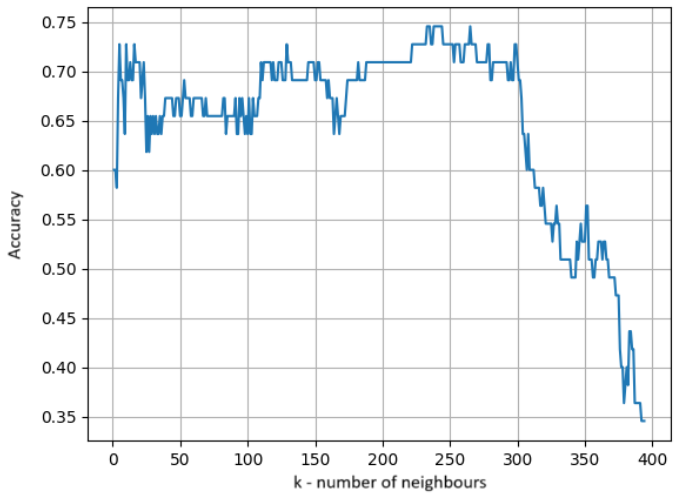
\includegraphics[width=1\linewidth]{ICS-5110-Fig-10.png}
    \caption{Accuracy scores of the k-NN model with different k values - training 70\%,  validation 10\% and testing 20\%}
    \label{fig:Accuracy scores of the k-NN model with different k values in training 70/10/20}
\end{figure}
\uline{\textbf{The accuracy peaked at k=231}} with a \uline{\textbf{value of 0.73.}}
Following we find the confusion matrix with K=231 regarding the prediction of the 55 validation points in TABLE V as well as the values of precision, recall and F1-Score for k=231 in TABLE VI.
\begin{table}
\centering
\begin{tabular}{p{0.12\linewidth}|p{0.15\linewidth}|p{0.15\linewidth}|p{0.15\linewidth}|p{0.15\linewidth}} \hline
&\textbf{L}&\textbf{M}&\textbf{H}\\ \hline
\textbf{L}&12&2&2\\ \hline
\textbf{M}&1&8&10\\ \hline
\textbf{H}&0&0&20\\ \hline
\end{tabular}
\caption{Confusion matrix for prediction of 55 validation points}
\label{tab:Confusion matrix for prediction of 55 validation points}
\end{table}
\begin{table}
\centering
\begin{tabular}{p{0.12\linewidth}|p{0.15\linewidth}|p{0.15\linewidth}|p{0.15\linewidth}|p{0.15\linewidth}} \hline
&\textbf{Precision}&\textbf{Recall}&\textbf{F1-score}\\ \hline
\textbf{L}&0.62&1.00&0.77\\ \hline
\textbf{M}&0.92&0.75&0.83\\ \hline
\textbf{H}&0.80&0.42&0.55\\ \hline
\textbf{Average values}&\textbf{0.78}&\textbf{0.72}&\textbf{0.72}\\ \hline
\end{tabular}
\caption{Performance metrics with k-NN and 20/10/70 split of the dataset in testing/validation/training sets}
\label{tab:Performance metrics with k-NN and 20/10/70 split of the dataset}
\end{table}
\\
\\
\textbf{III. Dataset split in training, validation and testing sets (64\%, 16\% , 20\%) - configuration evaluation against validation set}
The experiment has been continued by investigating how the percentage of the validation dataset would affect the value of accuracy. The size of the testing set is the same as the one defined in steps 1) and 2) of the experiment, for comparison purposes. The experiment setup has been amended so that:
\begin{itemize}
\item \uline{The dataset splitting was 20\% for testing, 16\% for validation and 64\% for training} Total 565 data points have been splitted in:
\SubItem{Number of datapoints in the training set: 361;}
\SubItem{Number of datapoints in the validation set: 91;}
\SubItem{Number of datapoints in the test set: 113;}
\item The \uline{Euclidean distance} has been applied as distance metric;
\item All points in each neighborhood have been weighted equally.
\end{itemize}
The experiment has been executed considering all numbers in the range [1, 361], in order to find the exact value of k where the accuracy reached the absolute maximum (Note that, the maximum value of the range for k has been reduced from 395 to 361 because now the number of datapoints in the training dataset has been reduced). The model has been trained with the training set and performance measured against the validation set. 
\begin{figure}
    \centering
    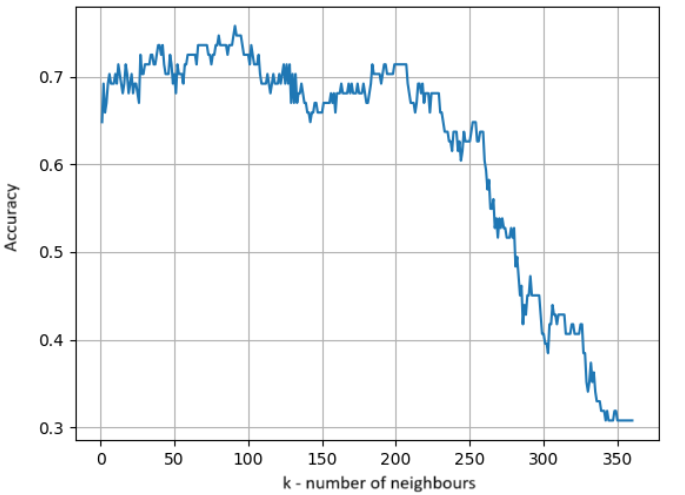
\includegraphics[width=1\linewidth]{ICS-5110-Fig-11.png}
    \caption{Accuracy scores of the k-NN model with different k values through cross-validation with training 64\%,  validation 16\% and testing 20\%}
    \label{fig:Accuracy scores of the k-NN model with different k values in training 64/16/20}
\end{figure}
\\
\uline{\textbf{The accuracy peaked at k=91}} with a \uline{\textbf{value of 0.76.}}
Following we find the confusion matrix with K=91 regarding the prediction of the 91 validation points in TABLE VII as well as the values of precision, recall and F1-Score for k=91 in TABLE VIII.
\begin{table}
\centering
\begin{tabular}{p{0.12\linewidth}|p{0.15\linewidth}|p{0.15\linewidth}|p{0.15\linewidth}|p{0.15\linewidth}} \hline
&\textbf{L}&\textbf{M}&\textbf{H}\\ \hline
\textbf{L}&25&5&3\\ \hline
\textbf{M}&4&14&10\\ \hline
\textbf{H}&0&0&30\\ \hline
\end{tabular}
\caption{Confusion matrix for prediction of 91 validation points}
\label{tab:Confusion matrix for prediction of 91 validation points}
\end{table}

\begin{table}
\centering
\begin{tabular}{p{0.12\linewidth}|p{0.15\linewidth}|p{0.15\linewidth}|p{0.15\linewidth}|p{0.15\linewidth}} \hline
&\textbf{Precision}&\textbf{Recall}&\textbf{F1-score}\\ \hline
\textbf{L}&0.70&1.00&0.82\\ \hline
\textbf{M}&0.86&0.76&0.81\\ \hline
\textbf{H}&0.74&0.50&0.60\\ \hline
\textbf{Average values}&\textbf{0.77}&\textbf{0.75}&\textbf{0.74}\\ \hline
\end{tabular}
\caption{Performance metrics with k-NN and 20/16/64 split of the dataset in testing/validation/training sets}
\label{tab:Performance metrics with k-NN and 20/16/64 split of the dataset}
\end{table}
\uline{Increasing the size of the validation set, the overall performance of the model has slightly improved}; this might be due to the fact that:
\begin{itemize}
\item a smaller training set may generalize predictions better resulting in improved accuracy. In fact, if the validation set is too small, it might not adequately represent the true distribution of the test data. By increasing the validation size, the model is tested on a more representative subset, leading to better generalization and higher test accuracy.
\item With k-NN, performance is sensitive to data distribution and hyperparameters. The increasing of the validation dataset size might have made the cross-validation more stable and provide a more reliable selection of k or other settings.
\end{itemize}
\textbf{IV. Experiment with the distance metrics}
The experiment went on checking whether different distance metrics would perform better than the Euclidean one, keeping the last experiment settings unchanged.
These are the results obtained using:
\begin{itemize}
\item \textbf{Manhattan distance:} The accuracy peaked at k=13 with a value of 0.73
\item \textbf{Glower’s distance:} The accuracy also peaked at k=13 with a value of 0.68
\end{itemize}
\uline{The results using the Manhattan and the Glower’s distances are lower than the ones obtained using the Euclidean distance metric and splitting the dataset in 20\% for testing, 16\% for validation and 64\% for training.}
\\
\\
\textbf{V. Final step of experiment and conclusions}
The experiments done until this point have been useful to fine-tune the model hyperparameters and to compare the different configurations results. 
The configuration of the k-NN model with better performance, evaluating it against the validation set, was the one described at step 3) of the experiments, where:

\begin{itemize}
\item \uline{A static split of the dataset has been applied with a ratio of 20\% for testing, 16\% for validation and 64\% for training}.
\item The \textbf{Euclidean metric} has been applied to calculate the distance between data points
\item The \textbf{accuracy} peaked at \textbf{k=91} with a value of \textbf{0.76}. With this number of neighbours to consider for the classification, the model performance metrics are:
\SubItem{Precision = 0.77}
\SubItem{Recall = 0.75}
\SubItem{F1-score = 0.74}
\end{itemize}
This configuration of the model didn’t have significant trade-off between precision and recall, meaning the model was neither overly cautious (high precision, low recall) nor overly aggressive (low precision, high recall). The model was stable and displayed a good balance between identifying positive instances and minimizing false alarms.\\
Once the best model was finalized, it was evaluated on the \textbf{test set} to measure its true generalization performance, that were the followings:
\begin{itemize}
\item \textbf{Accuracy = 0.69} 
\item \textbf{Macro average of the Precision = 0.69} 
\item \textbf{Macro average of the Recall = 0.67} 
\item \textbf{Macro average of the F1-score = 0.67} 
\end{itemize}
Such performance values of the model are also very similar to the ones obtained through the k-fold cross-validation: Accuracy of 0.69; F1-score = 0.68, confirming that the model should not overfit the dataset.
\\
\subsubsection{Implementation of the k-NN model} 
The following is a breakdown of the implementation of the k-NN model with best performance (see step 3 of the experiment):

\begin{itemize}
\item \textbf{Dataset preparation} 
















\item \textbf{Macro average of the Precision = 0.69} 
\item \textbf{Macro average of the Recall = 0.67} 
\item \textbf{Macro average of the F1-score = 0.67} 
\end{itemize}
\subsubsection{Model description} 
Naive Bayes is a set of supervised models that implement a statistical classification technique based on Bayes theorem. These are simple models that assume that the effect of a particular feature in a class is independent from other features. This precondition is met by our dataset which features are actually independent between each other, as depicted by the mutual information heatmap of Figure 1.\\
The Naive Bayesian model works with continuous features. Also this precondition is met because the features of the dataset had already been transformed from categorical to numerical and rescaled (the dataset has also been normalised).\\
The Bayes theorem calculates the conditional probability of a class $y_i$ given the features of the dataset X: 

\begin{displaymath}
P(y_i|X) = \frac{P(X|y_i) * P(y_i)}{P(X)}
\end{displaymath}

Where
\begin{itemize}
\item P($y_i$) is the probability of the i class to happen - the prior probability of $y_i$;
\item P(X): This is the probability of occurrence of features X, the evidence;
\item P($y_i$|X): the probability of the i class given that the given features - the posterior probability;
\item P(X|$y_i$): the probability of the features X given that the specific i class has occurred - the likelihood.
\end{itemize}
The Gaussian Naive Bayesian (GNB) model is the application of the Bayes theorem on conditional probability on a normally distributed data:
Considering the P(X) is equal for each class, only the numerator values are considered:

\begin{displaymath}
P(y_i|X) ∝ P(X|y_i) * P(y_i)
\end{displaymath}

Assuming that the features are independent between each others, then P(X|$y_i$) can be calculated as the product of the conditional probability of each feature given that the class it occurs:

\begin{displaymath}
P(X|y_i) = ∏_k P(x_k|y_i)
\end{displaymath}

Therefore

\begin{displaymath}
P(y_i|X) ∝ ∏_k P(x_k|y_i) * P(y_i)     ∏k P(x_k|y_i)
\end{displaymath}

Assuming that the features are normally distributed, the P($X_k$|$y_i$) follows a Gaussian distribution, which values of means and variances for each k feature and i class combination have been calculated during the training stage.

The prediction of the i class a new data point x' belongs to, is calculated by identifying the class with highest conditional probability value:

Predicted class for x' = Argmax [ P($y_i$|x') ]
\\
\subsubsection{Experiment execution} 
The goal of this experiment is to calculate the performance of the Gaussian Naive Bayesian model in order to have some comparison reference for the k-Nearest Neighbors (k-NN). 
For this reason, the same configuration that has brought the best performances for the k-NN model has been applied to the GNB model.
\uline{The dataset splitting was 20\% for testing, 16\% for validation and 64\% for training}. Total 565 data points have been splitted in: 
\begin{itemize}
\item Number of datapoints in the training set: 361
\item Number of datapoints in the validation set: 91
\item Number of datapoints in the test set: 113
\end{itemize}
\textbf{The accuracy of the Gaussian Naive Bayesian model is 0.64.}
The confusion matrix regarding the prediction of the 91 validation points is the following and these are the values of precision, recall and F1-Score:

\begin{table}
\centering
\begin{tabular}{p{0.12\linewidth}|p{0.15\linewidth}|p{0.15\linewidth}|p{0.15\linewidth}|p{0.15\linewidth}} \hline
&\textbf{L}&\textbf{M}&\textbf{H}\\ \hline
\textbf{L}&29&11&2\\ \hline
\textbf{M}&5&12&14\\ \hline
\textbf{H}&1&8&31\\ \hline
\end{tabular}
\caption{Confusion matrix for prediction of 91 validation points}
\label{tab:Confusion matrix for prediction of 91 validation pointsl}
\end{table}

\begin{table}
\centering
\begin{tabular}{p{0.12\linewidth}|p{0.15\linewidth}|p{0.15\linewidth}|p{0.15\linewidth}|p{0.15\linewidth}} \hline
&\textbf{Precision}&\textbf{Recall}&\textbf{F1-score}\\ \hline
\textbf{L}&0.66&0.78&0.71\\ \hline
\textbf{M}&0.83&0.69&0.75\\ \hline
\textbf{H}&0.39&0.39&0.39\\ \hline
\textbf{Average values}&\textbf{0.63}&\textbf{0.62}&\textbf{0.62}\\ \hline
\end{tabular}
\caption{Performance metrics with Gaussian Naive Bayesian model and 20/16/64 split of the dataset in testing/validation/training sets}
\label{tab:Performance metrics with Gaussian Naive Bayesian model and 20/16/64 split }
\end{table}


\subsection{Gradient Boosting Regressor}
\subsubsection{Introduction}
\subsubsubsection{I. Properties of the Data Set and Plan of Analysis}
The dataset used in this project, '\textit{ds\_salaries_\regression.csv}' \cite{Kaggle} contains salary-related information for data science roles. The dataset includes features such as job title, company location, experience level, company size, and remote ratio, among others. The goal is to predict salary values using machine learning models, specifically \acrfull{gbr}.

The plan of analysis involves:

\begin{itemize}
\item Loading and inspecting the dataset to understand its structure and quality.
\item Preprocessing the data, including the encoding of categorical variables, rescaling of numerical features, logarithmic transformation of salary data to manage skewness and guarantee non-negative predictions, and partitioning the dataset into training and testing subsets.
\item Building a scikit-learn pipeline integrating preprocessing and model training with the GBR model.
\item Evaluating the model's performance using cross-validation and metrics like  \acrshort{mae}.
\item Presenting the results through a Streamlit-based web application.
\end{itemize}


\subsubsubsection{II. Machine Learning Techniques Used}

The \acrshort{gbr} is a powerful ensemble technique that combines multiple weak learners, typically decision trees, to improve prediction accuracy \cite{friedman:greedy}. Key steps include:
\begin{itemize}
\item Encoding categorical variables with \textit{OneHotEncoder} and scaling numerical features with \textit{StandardScaler}.
\item Sequentially reducing the gradient of the loss function to improve accuracy.
\item Using a pipeline for seamless preprocessing and model training integration.
\item Optional hyperparameter tuning capability with parallel processing for advanced optimisation when required.
\item Implementing logarithmic transformation (log1p) of salary data to manage right-skewed distributions effectively, guarantee non-negative predictions, handle proportional salary changes appropriately, and enhance model performance across varying salary ranges.
\end{itemize}

\subsubsection{Background}
\subsubsubsection{I. Mechanics of Gradient Boosting Regressor}
The GBR builds an ensemble of decision trees sequentially, where each tree attempts to correct errors made by the previous one \cite{friedman:greedy}. The base model uses the following parameters:

\begin{itemize}
\item \textbf{Number of Trees} \textit{(n_estimators=500)}: Controls the number of boosting stages.
\item \textbf{Learning Rate} \textit{(learning_rate=0.05)}: Determines the contribution of each tree to the final prediction.
\item \textbf{Tree Depth} \textit{(max_depth=6)}: Controls the complexity of individual trees. 
\item \textbf{Other Parameters:} 
\SubItem{Minimum samples for a split \textit{(min_samples_split=5)}}.
\SubItem{Minimum samples in a leaf node \textit{(min_samples_leaf=4)}}.
\SubItem{Sub sampling ratio \textit{(subsample=0.8)}}.
\end{itemize}

For advanced usage, the model also supports hyperparameter tuning with an expanded parameter grid that includes:
\begin{itemize}
\item \textbf{Learning rates}: [0.01, 0.05, 0.1, 0.2].
\item \textbf{Number of trees}: [50, 100, 150, 300].
\item \textbf{Maximum tree depths}: [20, 25, 30, 35].
\item \textbf{Minimum samples split}: [2, 10].
\item \textbf{Maximum features}: [7, 15, 20].
\item \textbf{Minimum samples leaf}: [1, 4, 5, 6, 10].
\item \textbf{Subsample ratio}: [0.2, 0.4, 0.6, 0.8].
\end{itemize}

Gradient boosting reduces residual errors by fitting subsequent trees to the gradient of the loss function.

\subsubsubsection{II. Rescaling and Normalisation}
Numerical features (e.g., \textit{remote\_ratio}) are scaled using \textit{StandardScaler} to ensure equal contribution during training. Categorical variables are encoded using \textit{OneHotEncoder} with \textit{handle\_unknown='ignore'} and \textit{sparse\_output=FALSE} to prevent dimensionality issues.

The target variable (\texttt{Salary\_in\_USD}) undergoes logarithmic transformation using numpy\'s log1p function during training, with expm1 applied for inverse transformation during prediction. This mathematical transformation manages the right-skewed nature of salary distributions, ensures all predictions remain positive, prioritises relative (percentage) changes over absolute differences, and improves model accuracy across the full spectrum of salary ranges.

\subsubsubsection{III. Cross-Validation}
The model employs 5-fold cross-validation using KFold with \textit{shuffle=TRUE} and \textit{random\_state=42} to ensure robust evaluation. The scoring metric used is \textit{'neg\_mean\_absolute\_error'}, with cross-validation scores being calculated in the log-transformed space. The \acrshort{mae} is calculated for each fold, and both the average and standard deviation are reported to the user through the web interface.

\subsubsection{Data Preparation}
\subsubsubsection{I. Steps to Process the Dataset}
\begin{itemize}
\item Load the dataset using pandas.
\item Explore data to identify missing values and inconsistent entries.
\item Encode categorical variables using mappings (\texttt{experience\_level}, \texttt{employment\_type}, etc.) using predefined mappings and \textit{OneHotEncoder}.
\item Scale numerical features like \texttt{remote\_ratio}.
\item Split the dataset into training (80\%) and testing (20\%) subsets.
\end{itemize}

\subsubsubsection{II. Data Cleaning, Transformation, and Feature Engineering}
\begin{itemize}
\item \textbf{Data Loading:} Data is loaded and cached using Streamlit's \textit{@st\_cache\_data} decorator.
\item \textbf{Transformation:}
\SubItem{Experience level mapping (EN > Entry Level, MI > Mid Level, SE > Senior Level, EX > Executive).}
\SubItem{Employment type mapping (FT > Full-Time, PT > Part-Time, CT > Contract, FL > Freelance).}
\SubItem{Company size mapping (S > Small, M > Medium, L > Large).}
\SubItem{Target Variable Transformation: The salary values undergo logarithmic transformation (np.log1p) prior to model training, with predictions restored using inverse transformation (np.expm1). This methodology ensures positive predictions whilst properly handling the characteristically right-skewed distribution of salary data.}
\item \textbf{Feature Processing::} d
\SubItem{\textit{OneHotEncoder} for categorical features.}
\SubItem{\textit{StandardScaler} for numerical features.}
\end{itemize}

\subsubsection{Experiments}
\subsubsubsection{I. Description of Experiments}
The experiments include:
\begin{itemize}
\item Training the GBR with default parameters.
\item Tuning hyperparameters for optimal performance (e.g., \textit{learning rate, tree depth}).
\item Comparing performance across feature subsets and parameter combinations.
\end{itemize}

\subsubsubsection{II. Implementation of ML Techniques}
The model pipeline includes:
\begin{itemize}
\item A preprocessing step with \textit{ColumnTransformer} that applies \textit{OneHotEncoder} to categorical features and \textit{StandardScaler} to numerical features.
\item A \textit{GradientBoostingRegressor} configured with optimized parameters.
\item Logarithmic transformation of the target variable (salary), where training data undergoes log1p transformation and predictions are restored via expm1 transformation. This approach ensures heightened accuracy across all salary ranges.
\item Optional hyperparameter tuning functionality that:
\SubItem{Utilises parallel processing for parameter evaluation.}
\SubItem{Provides real-time visualization of tuning progress.}
\SubItem{Enables comprehensive parameter space exploration.}
\SubItem{Displays live updates of performance metrics.}
\end{itemize}

The model can be run in two modes:
\begin{itemize}
\item Standard mode with pre-optimised parameters.
\item Hypertuning mode for intensive parameter optimisation.
\end{itemize}

\subsubsubsection{III. Comparison of Results}
The model's performance evaluation encompasses several comprehensive metrics. The cross-validation analysis provides detailed insights through \acrfull{mae} scores across five folds, including both the average MAE and its standard deviation, offering a robust measure of model stability and accuracy.

Performance assessment is further strengthened through distinct training and testing MAE metrics, allowing for clear evaluation of the model's generalisation capabilities. These metrics are calculated on separate datasets to ensure unbiased performance measurement.

Feature importance is analysed and visualised through both numerical scores and an interactive bar chart, highlighting the top ten most influential features in the model's decision-making process. This analysis provides valuable insights into which factors most significantly impact salary predictions.

The model's configuration is thoroughly documented, detailing the core Gradient Boosting algorithm parameters including the number of trees, learning rate, tree depth specifications, sample split thresholds, leaf sample requirements, subsample ratio, and cross-validation methodology. This comprehensive information ensures full transparency of the model's architecture and training process.

The analysis was conducted using identical form parameters for both the standard and hypertuned models:

\begin{figure}
    \centering
    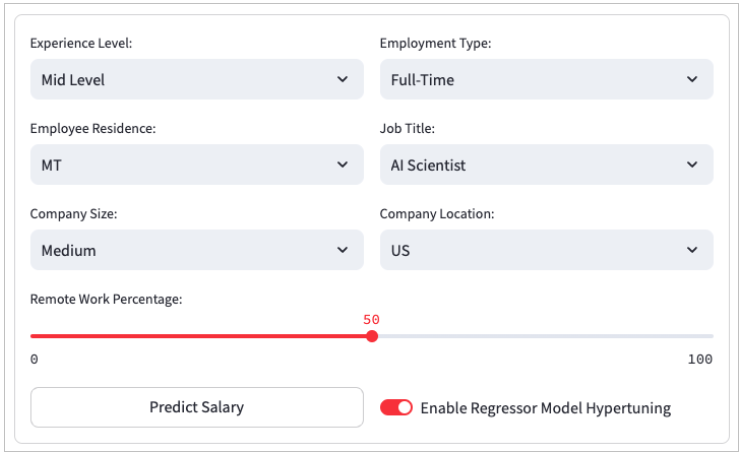
\includegraphics[width=1\linewidth]{ICS-5110-DataInput.png}
    \caption{Input Form Parameters}
    \label{fig:Input Form Parameters}
\end{figure}

These parameters were selected to provide a controlled comparison between the standard Gradient Boosting Regressor and its hypertuned variation. The only difference in execution was the activation of the hypertuning toggle, allowing for direct comparison of model performance and prediction outcomes.

A comparative analysis of the standard and hypertuned models revealed significant differences in both prediction behaviour and model performance:
\begin{itemize}
\item Prediction Variance:
\SubItem{The standard model demonstrated higher base predictions (\$100,181.87) compared to the hypertuned model (\$64,277.75).}
\SubItem{The hypertuned model showed more conservative predictions with narrower confidence intervals.}
\item Model Performance:
\SubItem{The hypertuned model showed more balanced MAE between training (\$25,039.82) and testing (\$26,649.45).}
\SubItem{The standard model displayed larger disparity between training (\$22,570.20) and testing (\$33,263.05) MAE, suggesting better generalisation in the hypertuned version.}
\item Parameter Optimisation:
\SubItem{Hypertuning significantly reduced the number of trees (from 500 to 150)}
\SubItem{Increased max tree depth (from 6 to 25).}
\SubItem{Reduced subsample ratio (from 0.8 to 0.2).}
\end{itemize}
These modifications resulted in a more efficient model with better generalisation capabilities.

\subsubsubsection{IV. Testing and Training Information}
The model maintains comprehensive documentation of its data structure and partitioning. This includes a detailed breakdown of the dataset size, showing the total number of records and their distribution between training and testing sets. The feature composition is clearly outlined, documenting the total number of features used in the model, with specific counts for both categorical and numerical variables. All this information is presented through a clear tabular interface, enabling users to fully understand the scale and composition of the data underlying the model's predictions.

\subsubsubsection{V. Model Information Display}
The model provides comprehensive information about its configuration and parameters through an interactive display that includes the core algorithm parameters. These encompass the model type (Gradient Boosting Regressor), number of trees (n\_estimators), learning rate, maximum tree depth, minimum samples split, minimum samples leaf, subsample ratio, and cross-validation configuration. All these metrics are displayed in real-time through the Streamlit interface, allowing users to understand the model's configuration and performance characteristics.

\subsubsubsection{VI. Parameter Modifications and Demographics}
The model offers flexibility in parameter handling through two approaches \cite{feurer:hyperparameter}
\begin{itemize}
\item \textbf{Standard Configuration:}
\SubItem{Fixed parameters optimised for general use cases.} 
\SubItem{Balanced for computational efficiency and accuracy.} 
\SubItem{Suitable for most prediction scenarios.} 
\SubItem{Consistent performance across different demographic segments.} 
\item \textbf{Advanced Tuning (Optional):}
\SubItem{Dynamic parameter adjustment through automated tuning.}
\SubItem{Parallel processing for efficient parameter space exploration \cite{feurer:hyperparameter}.}
\SubItem{Real-time monitoring of parameter effectiveness.}
\SubItem{Adaptable to specific demographic requirements.}
\end{itemize}
This dual approach ensures the model can serve both routine predictions and scenarios requiring more precise parameter optimisation.

\subsubsubsection{VII. Experimental Results}
The hypertuning process demonstrated notable improvements in model generalisation:
\begin{itemize}
\item Reduced overfitting as evidenced by closer training and testing MAE values.
\item More moderate predictions with narrower confidence intervals.
\item Computational efficiency through reduced number of trees.
\item Enhanced model robustness through optimised tree depth and sampling parameters.
\end{itemize}
These results suggest that hypertuning can be especially valuable for:
\begin{itemize}
\item Applications requiring high prediction reliability.
\item Scenarios where computational efficiency is vital.
\item Cases where model generalisation is important.
\end{itemize}

\subsubsection{Ethical Review}
\subsubsubsection{I. Ethical Aspects and Societal Implications}
\begin{itemize}
\item \textbf{Bias in Data:} Preprocessing steps address potential biases in historical salary data.
\item \textbf{Privacy:} Anonymised data prevents identification of individuals or companies.
\item \textbf{Fairness:} The model is designed to avoid reinforcing inequalities in salary prediction.
\end{itemize}

\subsubsection{Web Portal Usage Guide}
\subsubsubsection{I. User Guide}
\begin{itemize}
\item \textbf{Loading the Portal:} Access the Streamlit web application \cite{Streamlit}.
\item \textbf{Input Form:} 
\SubItem{\textbf{Dropdown Fields:}} 
\SubSubItem{Experience Level: Entry Level, Mid Level, Senior Level, or Executive.}
\SubSubItem{Employment Type: Full-Time, Part-Time, Contract, or Freelance.}
\SubSubItem{Job Title: Select from the list of unique titles in the dataset.}
\SubSubItem{Company Location: Select a location from the dropdown.}
\SubSubItem{Company Size: Choose Small, Medium, or Large.}
\SubItem{\textbf{Slider:} Adjust the remote_ratio percentage (0-100).} 
\SubItem{\textbf{Toggle:} Enable/Disable Hyperparameter Tuning (default disabled).} 
\item \textbf{Submit the Form:} Click "Predict Salary" to generate a salary prediction and range.
\item \textbf{Viewing Results:} 
\SubItem{\textbf{In Standard Mode:} (default)} 
\SubSubItem{Predicted salary range (\±15\% of base prediction).}
\SubSubItem{Base salary prediction in USD.}
\SubSubItem{Cross-validation results showing model performance.}
\SubSubItem{Model information table showing default parameters.}
\SubSubItem{Feature importance visualization.}
\SubItem{\textbf{In Hypertuning Mode:} (when enabled)} 
\SubSubItem{All standard mode outputs above plus:}
\SubSubItem{Real-time hyperparameter tuning progress.}
\SubSubItem{Live updates of parameter evaluation.}
\SubSubItem{Optimal parameter selection visualization.}
\end{itemize}

\subsubsubsection{II. Error Handling}
\begin{itemize}
\item Input validation ensuring all fields are filled before prediction.
\item Smooth handling of file loading errors.
\item Error catching during prediction process with user-friendly messages.
\item Automated salary transformation handling ensuring valid predictions through:
\SubItem{Logarithmic transformation during the training phase.}
\SubItem{Inverse transformation during prediction.}
\SubItem{Generation of valid, non-negative salary predictions.}
\end{itemize}



\subsection{Random forest Machine Learning}
\subsubsection{Introduction}
\subsubsubsection{I. Dataset Properties}
The dataset (i.e. '\textit{ds\_salaries.csv}') \cite{Kaggle} encompasses detailed information about salaries for various data science roles across geographies. Key features include:

\begin{itemize}
\item \textbf{Categorical variables:} job titles, employment types, company sizes, employee residences, and company locations.
\item \textbf{Numerical variables:} remote work ratio and salaries in USD.
\end{itemize}

This multidimensional dataset provides the foundation to construct a predictive machine learning model, offering valuable insights into salary determinants. By leveraging advanced regression techniques, this study aims to provide insights into salary prediction that could be instrumental for HR analytics and career planning for example.

\subsubsubsection{II. Analysis Framework}
\begin{itemize}
\item Data preprocessing:
\SubItem{Handle missing values.}
\SubItem{Encode categorical features.}
\SubItem{Split the dataset into training and testing sets.}
\item Develop a machine learning pipeline with a \acrfull{rfr}.
\item Assess model performance using metrics such as Mean Absolute Error, Mean Squared Error, R 2 Score, Cross Validation Scores.
\item Optimize the model via hyperparameter tuning using Parallelism for faster results.
\item Present findings through an interactive Streamlit interface.
\end{itemize}

\subsubsection{Background}
\subsubsubsection{I. Random Forest Regressor}
\newline
The \acrshort{rfr} is an ensemble learning method combining multiple decision trees, trained on random subsets of data and features. By averaging individual tree predictions, the RFR minimizes overfitting and ensures robust generalization \cite{breiman:forests}.

\subsubsubsection{II. Preprocessing Techniques}
\begin{itemize}
\item \textbf{Handling Missing Data}: Imputed with median values or removed if infrequent.
\item \textbf{Encoding Categorical Variables}:  Applied OneHotEncoder to translate job-related features into machine-readable formats.
\item \textbf{Feature Engineering}:  Interaction terms were added, and ordinal mappings were created for hierarchical data.
\end{itemize}

\subsubsubsection{III. Cross-Validation}
k-fold cross-validation was employed to ensure the model’s robustness. This technique splits the data into k subsets, iteratively training on k−1 folds and validating on the remaining fold. This ensures robustness in performance estimation and prevents overfitting during hyperparameter tuning \cite{hastie:elements}.

\subsubsection{Data Preparation}
\subsubsubsection{I. Cleaning and Transforming the Data}
\begin{itemize}
\item Missing data imputation was based on median values.
\item Encoding for features like experience levels was applied to ensure meaningful representation.
\item Feature interactions were engineered to capture potential non-linear relationships.
\end{itemize}

\subsubsubsection{II. Dataset Processing Workflow}
\begin{itemize}
\item Load and inspect the dataset.
\item Perform exploratory data analysis to identify outliers and distributions.
\item Encode categorical features and split the data into training (80\%) and testing (20\%) subsets.
\item Log Transformation of target variable to address the high variability in salary values and reduce the influence of extreme outliers. This ensures that the data is more evenly distributed and stabilizes the variance factor.
\item Rescaling and Normalization. While Random Forest is insensitive to feature scaling, preprocessing helps mitigate potential biases when combining distance-based algorithms in comparative studies.
\item Dimensionality Reduction and Feature Selection. These techniques improve computational efficiency and interpretability, especially when dealing with high-dimensional datasets.
\end{itemize}

\subsubsection{Python Implementation Methods}
\subsubsubsection{I. Modular Architecture}
\begin{itemize}
\item The script separates data preprocessing, training, tuning, and evaluation into modular functions.
\item The key modules in our Python script implementation include:
\SubItem{\texttt{ init() } : Prepares the pipeline and model.}
\SubItem{\texttt{ discover\_optimal\_params() }: Conducts hyperparameter tuning with grid search.}
\SubItem{\texttt{ predict() }: Generates predictions from user-provided inputs.}
\SubItem{\texttt{display\_stats()}: Visualizes evaluation metrics and dataset insights.}
\end{itemize}

\subsubsubsection{II. Preprocessing Steps}
\begin{itemize}
\item The script uses \texttt{ColumnTransformer} to preprocess features:
\SubItem{\textbf{Categorical Variables}: Encoded using \texttt{OneHotEncoder} (e.g., job titles, company size, etc...).}
\SubItem{\textbf{Numerical Variables}: Scaled with \texttt{StandardScaler} (e.g., remote work ratio).}
\item Log Transformation of Target:
\SubItem{The target variable (i.e. \texttt{Salary\_in\_USD}) was transformed with \texttt{np.log1p}. This reduced skewness by compressing large salary values and ensured that outliers had a less disproportionate effect on model training. The transformed target was used for training, and predictions were reverted to the original scale using \texttt{np.expm1} for evaluation.}
\SubItem{Splitting of the dataset into training (80\%) and testing (20\%) subsets with the use of \texttt{train\_test\_split()} method.}
\end{itemize}


\subsubsubsection{III. Model Pipeline}
\begin{itemize}
\item Combines preprocessing and modelling in a Pipeline \texttt{Pipeline}.
\item The \texttt{RandomForestRegressor} which gets initialized with either default or tuned hyperparameters, depending on the mode of execution (dynamically set form the UI).
\end{itemize}

\subsubsubsection{IV. Hyperparameter Tuning}
\begin{itemize}
\item We used \texttt{ParameterGrid} to outline possible parameter combinations:
\SubItem{Number of estimators (\texttt{n\_estimators}).}
\SubItem{Maximum tree depth (\texttt{max\_depth}).}
\SubItem{Minimum samples per leaf (\texttt{min\_samples\_leaf}).}
\SubItem{Maximum features per split (\texttt{max\_features}).}
\item Leveraging parallel processing via \texttt{joblib.Parallel} to optimize computational efficiency during our \texttt{GridSearchCV} implementation.
\end{itemize}

\subsubsubsection{V. Model Evaluation}
\begin{itemize}
\item Predictions are transformed back to the original scale using \texttt{np.expm1} to ensure evaluation metrics like MAE, MSE, and $R^2$ are calculated on interpretable salary values.
\item Calculating several key metrics for performance evaluation:
\SubItem{\textbf{Mean Absolute Error (MAE)}: Measures average prediction error.}
\SubItem{\textbf{Mean Squared Error (MSE)}: Penalizes larger deviations.}
\SubItem{\textbf{ $R^2$ Score}: Quantifies the goodness of training.}
\item Employing k-fold cross-validation to ensure generalization.
\end{itemize}

\subsubsubsection{VI. Feature Importance Analysis}
\begin{itemize}
\item Extracting feature importances using the fitted Random Forest model.
\item Finally displaying the top 10 features influencing our salary predictions output. 
\end{itemize}

\subsubsubsection{VII. Streamlit Integration}
\begin{itemize}
\item This was used to provide a user-friendly interface for:
\SubItem{Accepting user input and preferences.}
\SubItem{Visualizing hyperparameter tuning progress.}
\SubItem{Interpreting model results through charts and tables.}
\SubItem{Generating real-time predictions from user-provided inputs.}
\end{itemize}

\begin{figure}
    \centering
    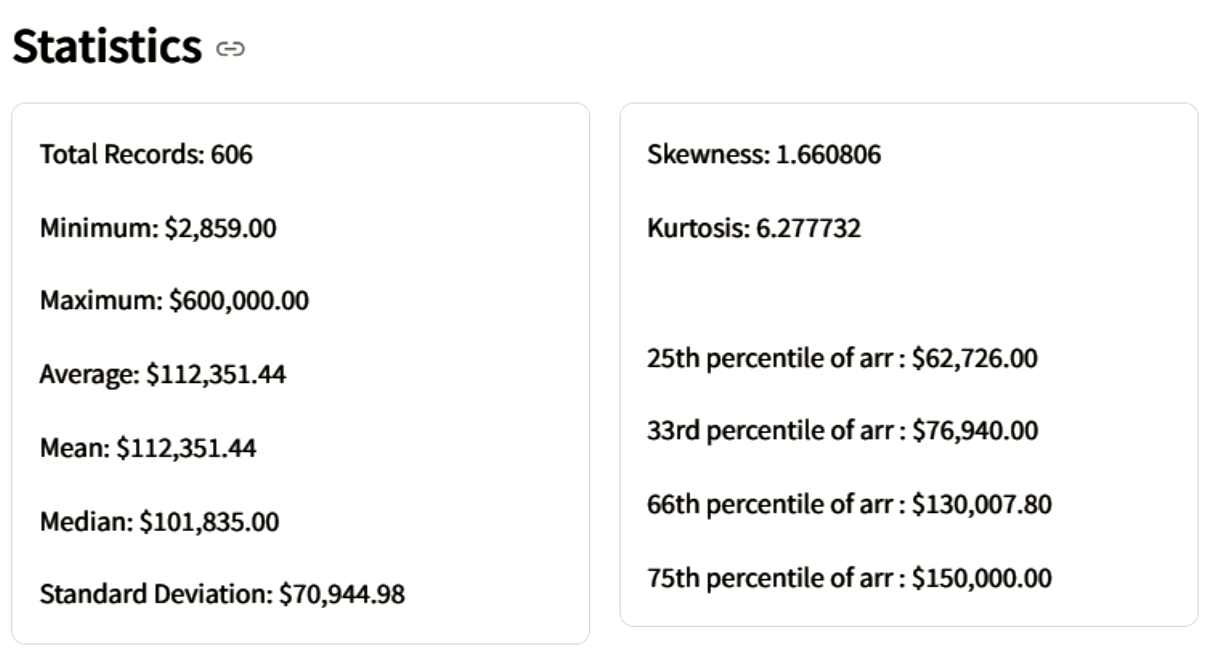
\includegraphics[width=1\linewidth]{ICS-5110_website_stats.png}
    \caption{Statistical overview of the Data-set}
    \label{fig:Statistical overview of the Data-set}
\end{figure}

\subsubsection{Experiments}
\subsubsubsection{I. Experimentation Design}
Three experiments were conducted:
\begin{itemize}
\item Baseline performance evaluation with default RFR parameters.
\item Model performance after hyperparameter tuning.
\item Assessment of model behaviour using subsets of features to identify key predictors.
\end{itemize}

\subsubsubsection{II. Hyperparameter Tuning}
Hyperparameter optimization employed an implementation of \texttt{GridSearchCV} with cross-validation. Parameters that we decided to tune included:
\begin{itemize}
\item \textbf{Number of Estimators}: Attempted to improve accuracy until around 300 estimators. (For the purpose of this experiment to keep it running in a short timeframe, the actual set space values were only 50, 100, 150, 300)
\item \textbf{Max Depth}: Adjusting this enable us to control overfitting and improved predictions for senior roles. (Again, for the same purpose as the previous one, we kept a limited value space for this parameter, mainly 20, 25, 30, 35)
\item \textbf{Other Parameters}: \texttt{max\_features}, \texttt{min\_samples\_split}, and \texttt{min\_samples\_leaf} were also automatically fine-tuned.
\end{itemize}

\subsubsubsection{III. Results}
Optimal parameters that yielded the lowest MAE, following a parameter hyptertuning procedure, where:
\begin{itemize}
\item \texttt{max\_depth=30}
\item \texttt{max\_features=15}
\item \texttt{min\_samples\_leaf=1}
\item \texttt{min\_samples\_split=10}
\item \texttt{n\_estimators=100}
\end{itemize}
The log transformation effectively stabilized the target variable by reducing the impact of extreme salary values. This improved the model's ability to generalize and lowered the MAE from \textbf{\$34,655.20} to \textbf{\$27,565.34}. Despite the improvement, the MAE remains relatively high due to the inherent variability in salaries.
\begin{figure}
    \centering
    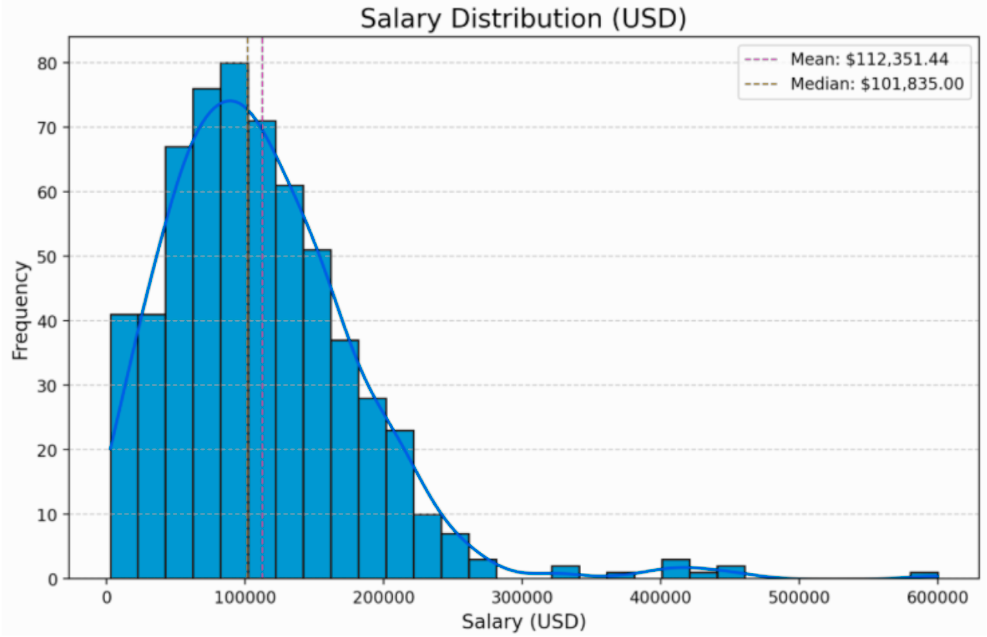
\includegraphics[width=1\linewidth]{ICS-5110_salary_distrobution.png}
    \caption{Salary distribution of the Data-set}
    \label{fig:Salary distribution of the Data-set}
\end{figure}

\subsubsection{Ethical Considerations}
\subsubsubsection{I. Bias Mitigation}
The model addressed potential biases by balancing under-represented categories, such as remote work ratios or rare job titles. These measures aimed to prevent overfitting to majority categories.
\subsubsubsection{II. Transparency}
Caveats were clearly communicated:
\begin{itemize}
\item Reliance on historical data limits predictions’ future applicability.
\item Predictions should complement, not replace, human decision-making.
\end{itemize}


\subsubsection{Results and Insights}
The Mean Absolute Error (MAE) is a metric that quantifies the average magnitude of errors in predictions made by a machine learning model. In our case, the MAE was that of \textbf{\$27,565.34} which means that, on average, our salary predictions made by the RFR deviate from the actual salaries by approximately \textbf{\$27,565.34}. 
\\
The addition of the log transformation reduced the skewness in salary values. The model's predictions were less influenced by extreme values, providing more balanced error measurements. The MAE, evaluated on the original salary scale, remains high due to the inherent variability in the dataset. Also, adding more data would drastically increase the performance.
\subsubsubsection{I. Implications of the MAE Value}
An MAE of \$27,565.34 is relatively large in the context of a salary prediction task. This may indicate that the model is not performing as well as one would hope in predicting accurate salaries. To verify this, we calculated the average salary in our dataset, together with some other statistics, to see if this is significantly lower than our MAE value.

With a total average salary of \$112,351.44, we concluded that this is significantly higher than our MAE of \$27,565.34 making our predictions off by approximately 24.54\% of the total average salary in the dataset. While the error is not negligible, it is less concerning and the reason for this high MAE may be coming from not having enough data.

\begin{figure}
    \centering
    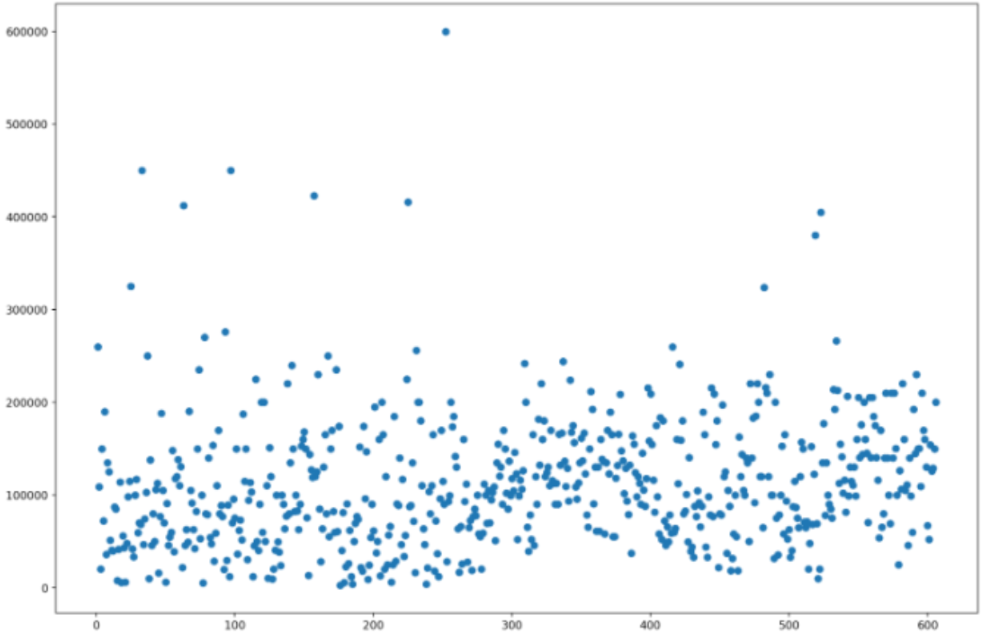
\includegraphics[width=1\linewidth]{ICS-5110_scatterplot.png}
    \caption{Scatter Plot of the Dataset entries}
    \label{fig:Scatter Plot of the Dataset entries}
\end{figure}

A large standard deviation value (i.e. \$70,944.98) indicates high variability in total salaries. Salaries range widely from a minimum of \$2,859 to a maximum of \$600,000, suggesting the presence of outliers or extreme values.

In addition, the histogram plot in Screenshot 1 reveals a right-skewed distribution, where a small number of extremely high salaries are inflating the mean. The median (i.e. \$101,835) is less than the mean (i.e. \$112,351.44), confirming this skewness. Extremely high salaries, like the \$600,000 figure, are potentially distorting our model performance by contributing disproportionately and inflating our MAE.

\subsubsection{Improvements and Future Work}
\begin{itemize}
\item \textbf{Training Separate Models}: Training separate models for different salary groups (i.e. Low, Medium, High) might reduce the variability within each class segment.
\item \textbf{Incorporating More Data}: More data in our dataset would definitely help to improve predictive accuracy.
\end{itemize}




\subsection{Support Vector Machine - Danou}
\begin{itemize}
\item \hint{describe the mechanics of the selected machine learning techniques}
\item \hint{Describe experiment}
\item \hint{Describe implementation of the ML technique}
\item \hint{Assess how modification in the parameters or cost functions can affect the output}
\item \hint{Describe model evaluation by calculating the applicable performance parameters:}
\end{itemize}


\section{Results comparison}
\textbf{Classifiers results comparison - k-NN vs Gaussian Naive bayesian}
The following table summarizes the performance metrics for the k-NN and the Gaussian Naive Bayesian model that have been applied to the same dataset using the same configurations.

\begin{table}
\centering
\begin{tabular}{p{0.12\linewidth}|p{0.15\linewidth}|p{0.15\linewidth}|p{0.15\linewidth}|p{0.15\linewidth}} \hline
\textbf{Model}&\textbf{Accuracy}&\textbf{Precision}&\textbf{Recall}&\textbf{F1-score}\\ \hline
\textbf{k-NN}&0.69&0.69&0.67&0.67\\
\textbf{GNB}&0.64&0.63&0.62&0.62\\
\hline\end{tabular}
\caption{Comparison of the performance metrics of the k-NN and the Gaussian Naive Bayesian models applying the same 20/16/64 split of the dataset}
\label{tab:Comparison of the performance metrics of the k-NN and the Gaussian Naive Bayesian models}
\end{table}
The k-NN performs better than the Gaussian Naive Bayesian model, because it provides a level of configurability of its hyperparameters that GNB doesn’t have. This allowed to tune the model with the best value of k-neighbours that maximizes the accuracy performance of the model.
\\
Another reason that could explain why the k-NN model results to perform better than the Gaussian Naive Bayesian model in every aspect, might be that the Gaussian Naive Bayesian model assumes that the features follow a normal distribution and are fully independent. The dataset doesn’t fully meet such requirements, in fact, even if the dataset has been normalised and the features display a good level of independence between each other, they are not totally independent between each other and this can negatively affect the performance of the GNB model.
\hint{Regression models results comparison}
\hint{xxxxxx}


\section{Ethical review}
\subsection{Data Source and Integrity}
The dataset has been taken from one of the public domain datasets provided by \href{https://www.kaggle.com/datasets/ruchi798/data-science-job-salaries}{www.kaggle.com}.\\
The source of the dataset mentioned in Kaggle is the ai-jobs.net website (a global digital media \& technology company based in Zürich, Switzerland). However, it has to be highlighted that the URL provided as source (\href{https://salaries.ai-jobs.net/}{salaries.ai-jobs.net}) in Kaggle is not reachable, so this detail cannot be confirmed.\\
The \href{https://www.kaggle.com/ruchi798/datasets}{Kaggle user} who provided the dataset is a “Dataset Grandmaster” on Kaggle, meaning that she has provided valuable and good quality datasets so far on the website.\\
The data analysis has not highlighted any peculiarity of the dataset that might raise concerns on its reliability, however, it must be said that the dataset metadata provided in Kaggle is not accurate enough to be 100\% sure that the dataset is reliable.
\subsection{Data Bias}
The data regards roles that belong to the Data science and machine learning job market umbrella, under different types of contracts and linked to companies of different sizes and located in about 50 different countries. The data regards the Covid and early post-Covid period (from 2020 to 2022) and this is also reflected on the fact that most of the positions of the dataset are remote and hybrid ones. In conclusion, it is admissible to say that the data is representative of the population it is supposed to serve.\\
The data analysis has highlighted that most of the data regards companies located in the USA and workers resident in the USA. While this can be a realistic representation of this specific job market, that is mainly centered in the USA, it could also be considered as a sampling bias that can lead to the over representation of a certain group (in this case companies located and workers residents in the USA). 
\subsection{Data Privacy}
The dataset does not include any sensitive or \acrfull{pii} data.
\subsection{Transparency and Accountability}
The machine learning models applied to this dataset have been described in this report and they are also made available online on GitHub for transparency. The authors of this report are accountable for the models’ predictions.
\subsection{Fairness and Equity}
The prediction of a salary for a job in the Data Science and Machine learning job market might result in any unfair treatment of individuals if it is used as leverage to bargain a better salary during the contract negotiation stage. The candidates who don’t have access to this tool and information,might be disadvantaged compared to those who have access to it.  
\subsection{Social Impact}
The deployment of the models described in this report can help navigate the job market in the Data science and Machine learning area, providing an understanding of the expected salary ranges based on the level of  experience and the job title of interest, giving an indication on what type of contract and company size would fit better each individual career path.  
\subsection{Environmental Impact}
The dataset size and the models computational requirements don’t pose relevant environmental costs. 
\subsection{Accessibility}
The Web tool that allows us to interact with the prediction models described in this report will be publicly accessible here: 
\hint{https://ics5110-group-assignment-u6ufn8qggyaoxompbbokzy.streamlit.app/}
However, the web tool is \uline{not} designed in an accessible manner, and it doesn’t follow usability principles that make the web tool accessible to people with disabilities. 
\subsection{Consent and Opt-In}
The deployment of the models don’t require consent from the end-users for data collection or tracking.

\section{Web portal usage guide}
This guide provides instructions for using our data analysis web portal, which allows users to explore and analyse employment data, including salary insights and predictions.

\subsection{Accessing the Portal}
\begin{itemize}
\item Launch the web portal through your preferred web browser
\item Navigate to: \hint{https://ics5110-group-assignment-u6ufn8qggyaoxompbbokzy.streamlit.app/}
\item The system will automatically initialise all necessary components
\item You'll be presented with the main interface once loading is complete
\end{itemize}

\subsection{Key Features}

\subsubsection{Data Fields Filling Options}
The portal allows the user to fill in the form based on several parameters:
\begin{itemize}
\item \textbf{Experience Level}: Select your level of professional experience
\item \textbf{Employment Type}: Choose between different employment arrangements
\item \textbf{Location Details}: 
\SubItem{\textbf{Employee Residence}: Select where you currently reside}
\SubItem{\textbf{Company Location}: Specify the company's location}
\item \textbf{Job Information}: 
\SubItem{\textbf{Job Title}: Select specific job roles}
\SubItem{\textbf{Company Size}: Filter by organisation size}
\item \textbf{Remote Work}: Adjust the remote work ratio using the provided slider
\end{itemize}

\subsubsection{Analysis Features}
\begin{itemize}
\item \textbf{Regression Analysis}: 
\SubItem{Access detailed salary predictions based on selected parameters}
\SubItem{View statistical correlations between different employment factors}
\SubItem{Analyse salary trends across different demographics}
\item \textbf{Classification Analysis}: 
\SubItem{Explore categorical insights about employment patterns}
\SubItem{View grouped data based on selected filters}
\SubItem{Understand distribution across different employment categories}
\end{itemize}

\subsubsection{Advanced Options - Hypertuning Feature}
\begin{itemize}
\item Enable/disable hyperparameter tuning for more accurate predictions
\item Recommended for detailed analysis requirements
\item May increase processing time but provides more precise results
\item Allow processing time when hypertuning is enabled
\end{itemize}

\subsection{Using the Portal}
\begin{itemize}
\item \textbf{Setting Up Your Analysis}: 
\SubItem{Begin by selecting relevant filters from the sidebar}
\SubItem{Ensure all required fields are populated}
\SubItem{Adjust the remote work ratio as needed}
\item \textbf{Generating Insights}: 
\SubItem{Click the "Predict" button to generate analysis}
\SubItem{Wait for the system to process your request}
\SubItem{Review the generated visualisations and insights}
\SubItem{All calculations are performed in real-time}
\item \textbf{Interpreting Results}: 
\SubItem{Examine the presented graphs and charts}
\SubItem{Review statistical information provided to explore different aspects of the data}
\item \textbf{Data Exploration}: 
\SubItem{Use different combinations of filters to understand trends}
\SubItem{Compare results across different job titles and locations}
\end{itemize}






\section{Conclusions}
\hint{This paragraph will end the whole thingy}


\clearpage

\appendix
%Appendix A
%ACKNOWLEDGMENTS are optional
\section{Acknowledgments}
This section is optional; it is a location for you
to acknowledge grants, funding, editing assistance and
what have you.  

\section{Headings in Appendices}
The rules about hierarchical headings discussed above for
the body of the article are different in the appendices.

\setglossarystyle{list} 
\printglossary[type=\acronymtype]

\listoffigures  % Listing Images
\listoftables   % Listing Tables
\listoflistings % Listing Code

\bibliographystyle{abbrv}
\bibliography{sigproc}  % sigproc.bib is the name of the Bibliography in this case
% You must have a proper ".bib" file
%  and remember to run:
% latex bibtex latex latex
% to resolve all references
    
\end{document}